\providecommand{\myrootdir}{..}
\documentclass[\myrootdir/main.tex]{subfiles}

\begin{document}

\chapter{Empirical Comparison Study}
\label{sec:study}
To investigate when PBE, CTS and KWS are suited to retrieve chunks from CI build logs we evaluated our implementation of those techniques on the \emph{Failing Build Log Data Set}.
This chapter describes our study design, the analysis of the study results and threats to the validity of our conclusions.
The analysis of the study results first focusses on each of the three techniques and describes how each one performs best.
Later we compare them against each other and describe their trade offs against each other.
This chapter answers our second research question and its subquestions:
\begin{simplebox}{Research Questions}
\begin{itemize}
  \item[\textbf{RQ2:}] When are PBE, TS, and SKWS suited to retrieve information from CI build logs?
  \item[\textbf{RQ2.1:}] How many examples do PBE, TS, and SKWS need to perform best?
  \item[\textbf{RQ2.2:}] How accurate are the retrievals of PBE, TS, and SKWS?
  \item[\textbf{RQ2.3:}] How structurally similar do the examples for PBE and TS need to be for the techniques to be applicable?
\end{itemize}
\end{simplebox}

\begin{figure}[htbp]
	\centering
	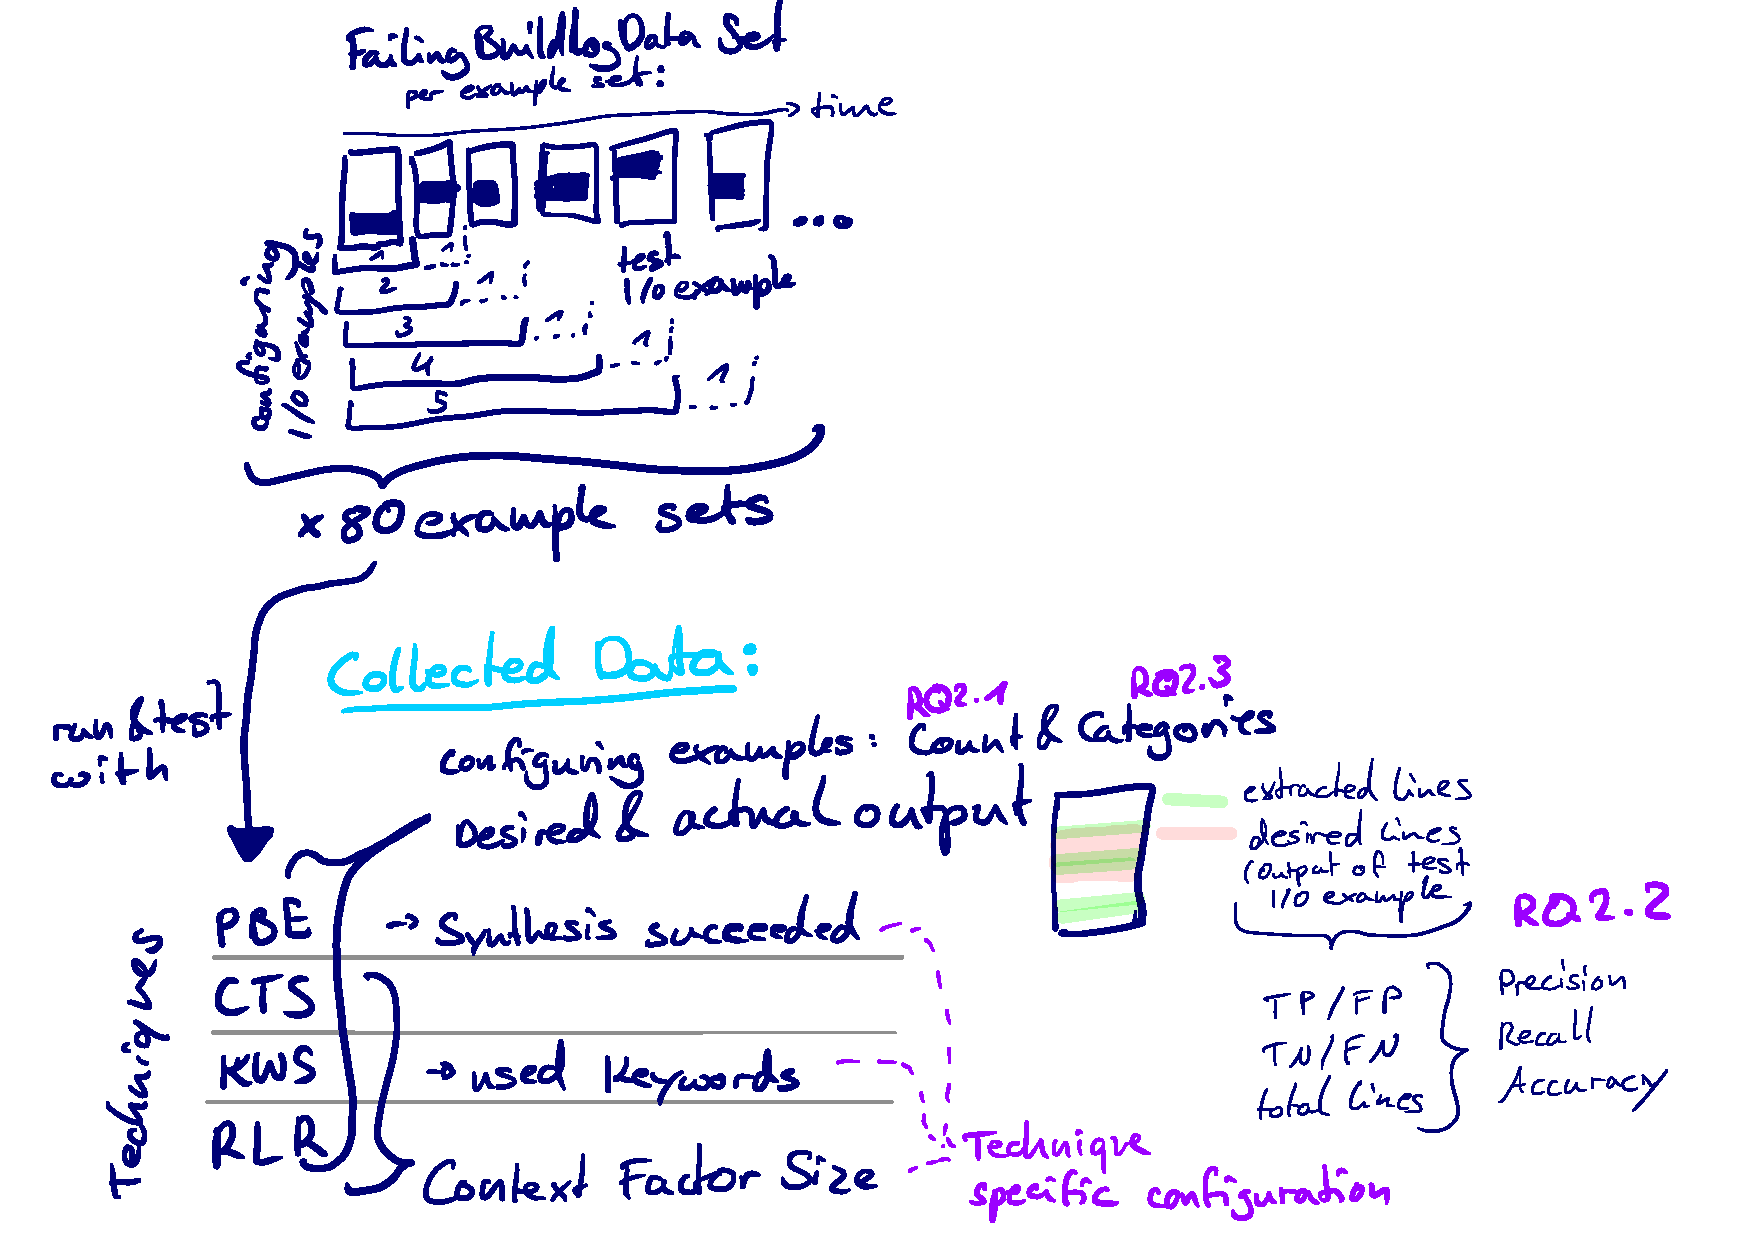
\includegraphics[width=\textwidth, clip]{img/study-design.pdf}
	\caption{Study Design of our technique comparison study}
	\label{fig:study}
\end{figure}

\section{Study Design}
For the comparison study we evaluate the three chunk retrieval techniques PBE, CTS and KWS, described in Sections \ref{sec:expl-pbe},\ref{sec:expl-ts} and \ref{sec:expl-skws}.
RLR, explained in Section \ref{sec:expl-rlr}, acts as a baseline for the comparison.
We run four techniques on the example sets from the \emph{Failing Build Log Data Set}.

The examples are sorted chronologically, i.e. a technique is configured with examples from the directly preceding build logs.
For each example set and each technique, we select one to five successive I/O examples as configuration, the \emph{configuring I/O examples}, and run the chunk retrieval on the next I/O example, the \emph{test I/O example}.

For each of our evaluation runs we measure the desired vs. actual output lines of the chunk retrieval.
The desired output is given by the output of the test I/O example, which acts as the oracle for our evaluation.
From this we obtain true/false positives/negatives and calculate precision, recall and accuracy, which we use to answer \textbf{RQ2.2}.
We register the number of examples used as configuration for each run to answer \textbf{RQ2.1} and their structural categories to answer \textbf{RQ2.3}.


%taking The Failing Build Log Data Set - run 3(4 with random) techniques with increasing example count - measuring xyz - justify choices like running chronologically / testing on 1 example / no k-fold validation - how are keywords for the search selected?

\section{Analysis}
This section presents the evaluation results for PBE, CTS and KWS separately and discusses under which circumstances these techniques yield best results.
Afterwards it compares the three techniques with each other and RLR as baseline.
The section concludes with recommendations on which technique is suited for different situations.

% \begin{figure}[htbp]
% 	\centering
% 	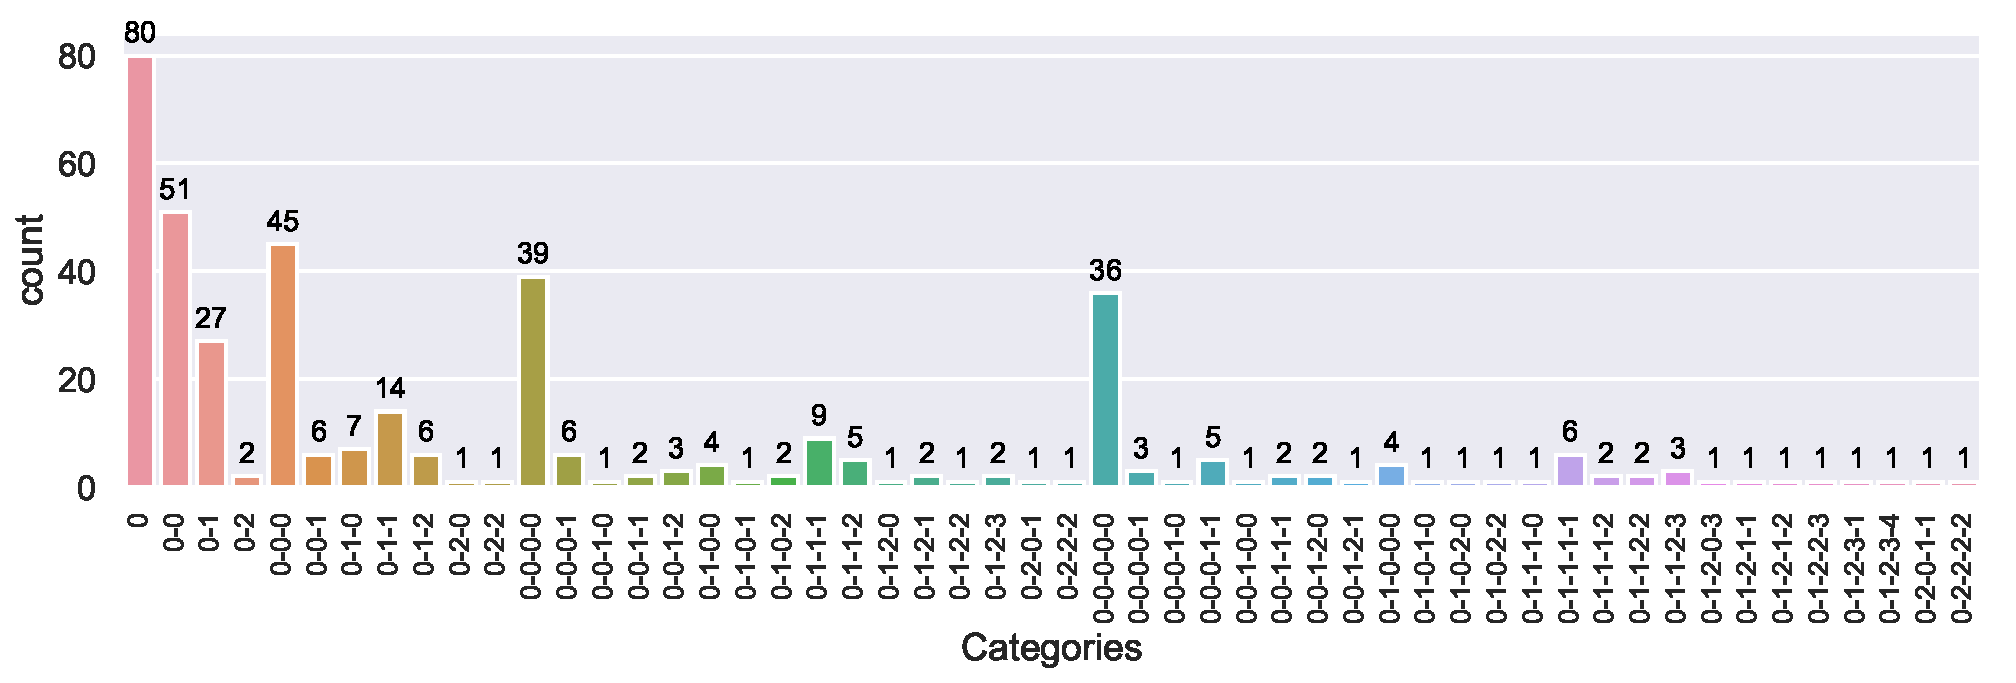
\includegraphics[width=\textwidth, clip]{img/big-study/categories-dataset.pdf}
% 	\caption{Distribution of Category Combinations in the Example Sets used for Configuration in our Study}
% 	\label{fig:categories-dataset}
% \end{figure}

% \begin{figure}[htbp]
% 	\centering
% 	\begin{minipage}{0.45\textwidth}
% 		\centering
% 		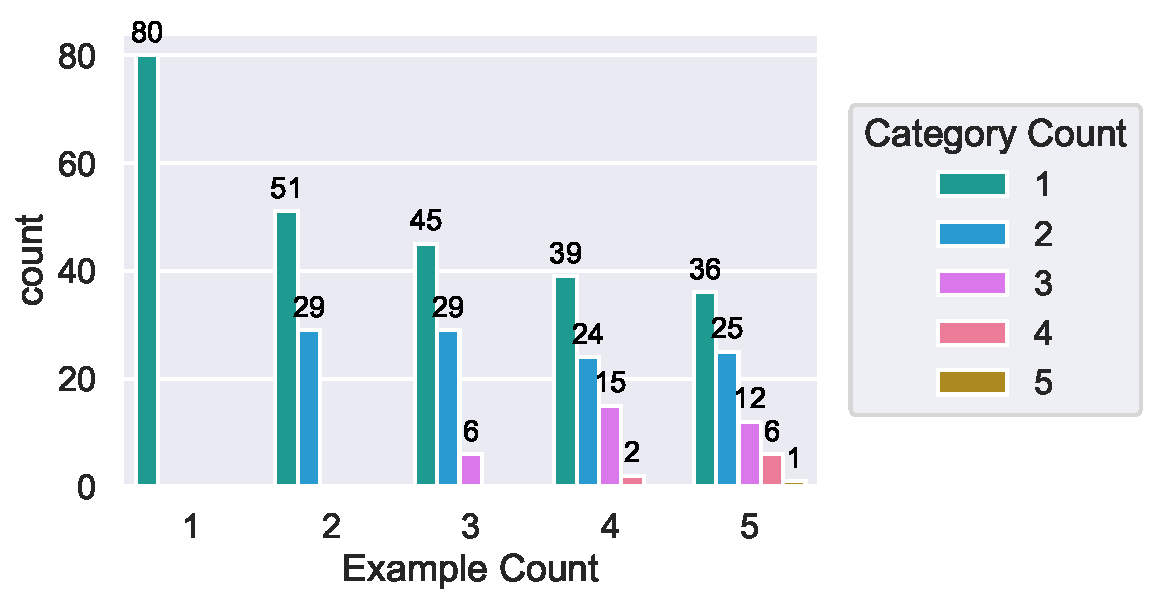
\includegraphics[width=\textwidth, clip]{img/big-study/categorycount-examplecount-dataset.pdf}
% 		\caption{Distribution of the Count of Categories within the Examples used for Configuration in our Study}
% 		\label{fig:categorycount-examplecount-dataset}
% 	\end{minipage}\hfill
% 	\begin{minipage}{0.45\textwidth}
% 		\centering
% 		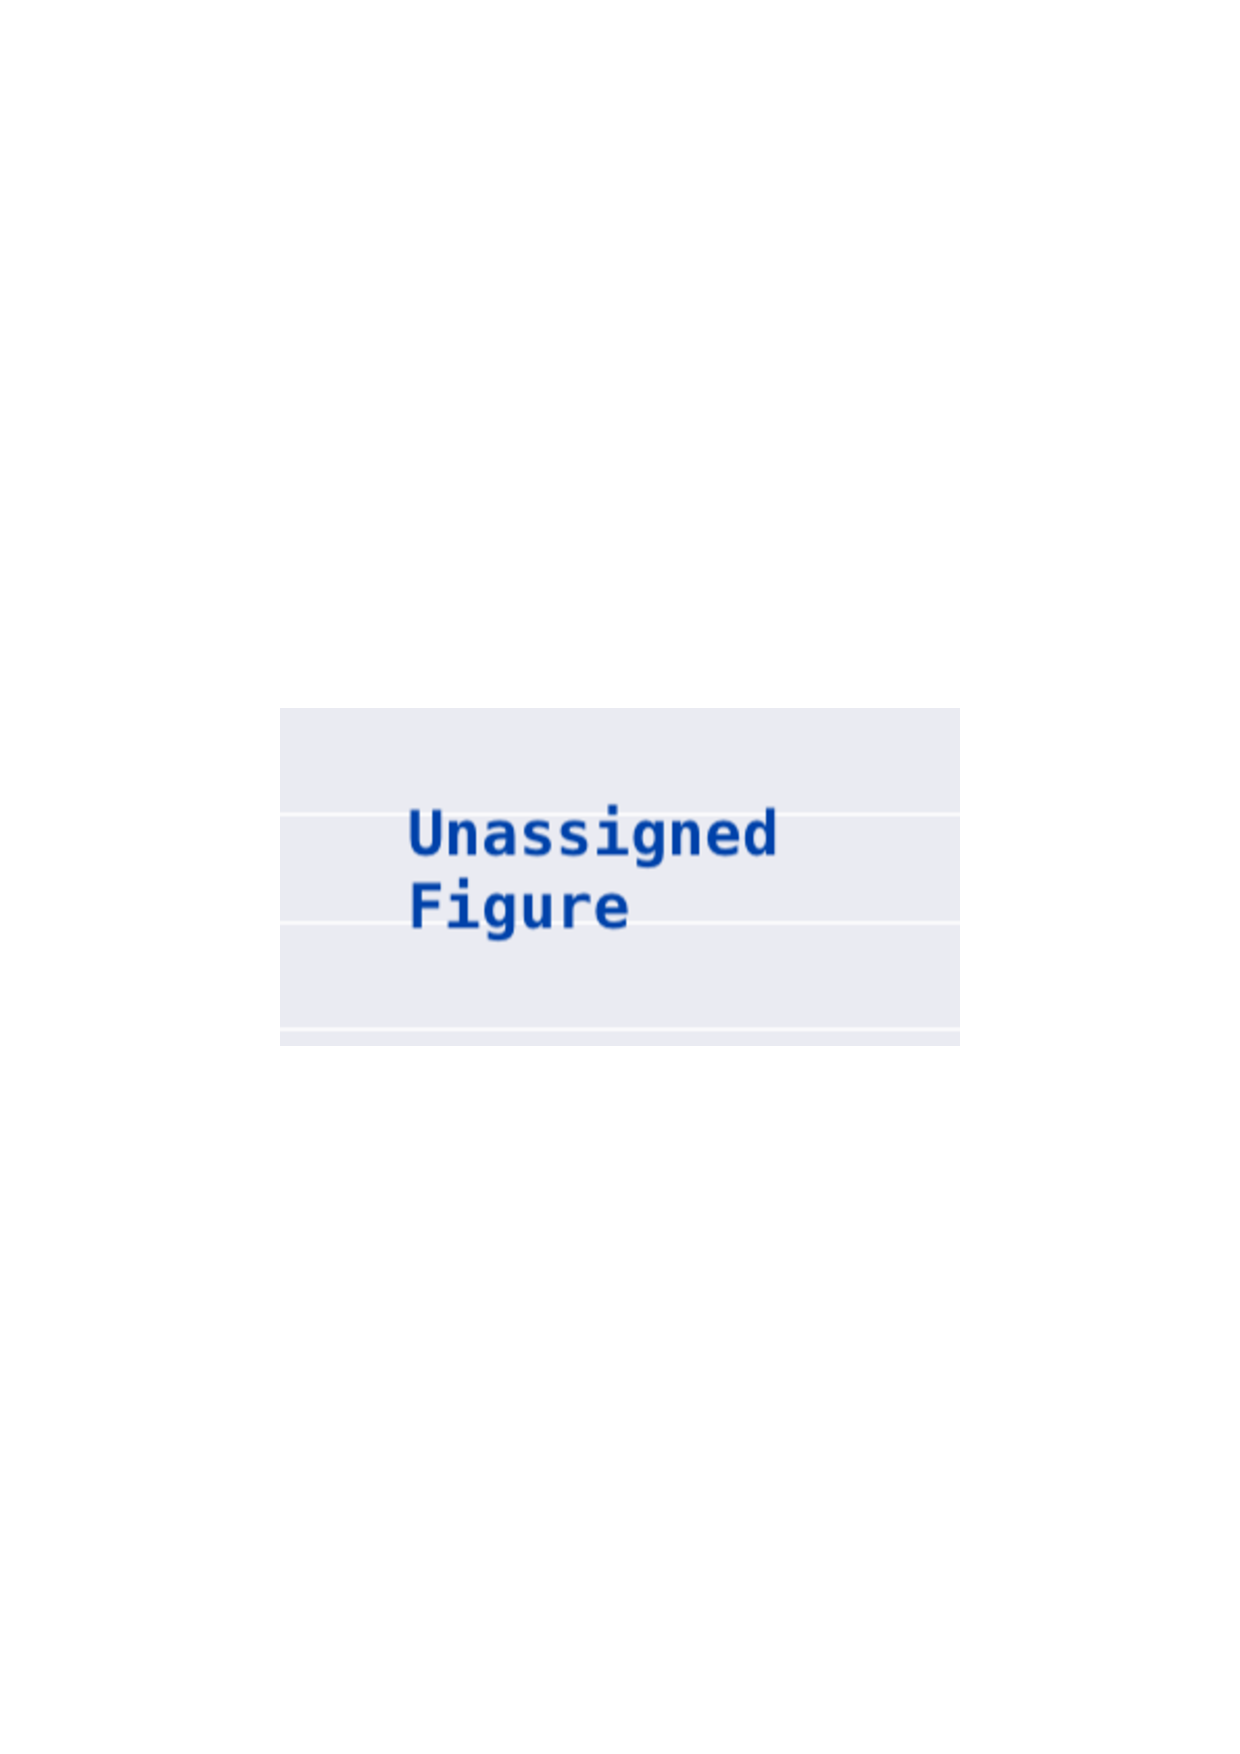
\includegraphics[width=\textwidth, clip]{img/big-study/xxx.pdf}
% 		\caption{caption}
% 		\label{fig:xxxy}
% 	\end{minipage}
% \end{figure}

% \subsection{Category Distribution in Data Set}
% Categories distributed in over data set
% - why are we looking at that?: interesting how categories are distributed for this real world example of build Failure reasons in travis ci categorization
% - Figure \ref{fig:categories-dataset} shows the distribution of categories in the configuring example sets in rou study
% - Figure \ref{fig:categorycount-examplecount-dataset} shows the category count separated by the different example count.


\begin{figure}[htbp]
	\centering
	\begin{minipage}{0.45\textwidth}
		\centering
		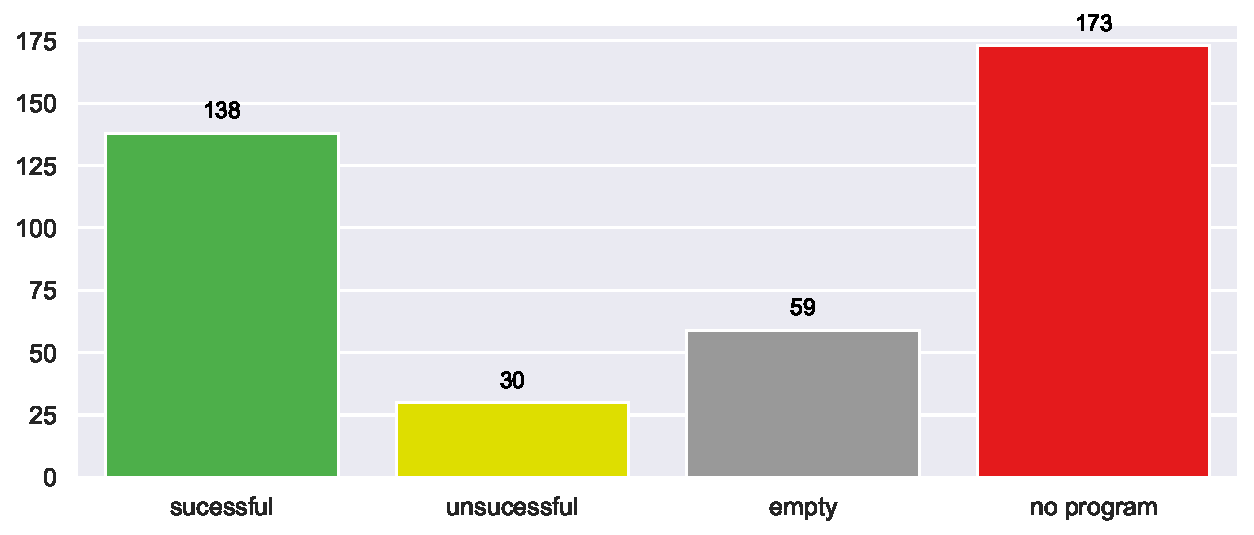
\includegraphics[width=\textwidth, clip]{img/big-study/failure-reason-PBE.pdf}
		\caption{Success of Chunk Retrieval Runs with PBE}
		\label{fig:failure-reason-PBE}
	\end{minipage}\hfill
	\begin{minipage}{0.45\textwidth}
		\centering
		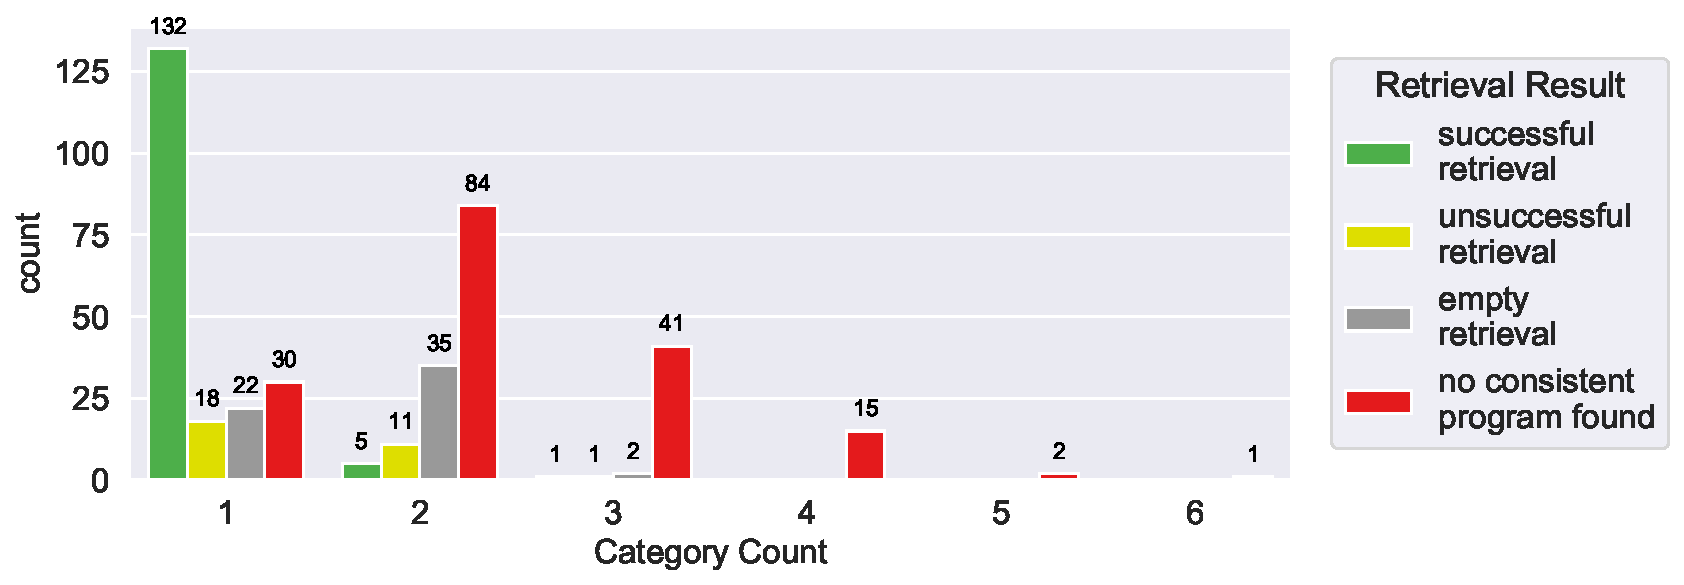
\includegraphics[width=\textwidth, clip]{img/big-study/failure-reason-categorycount-PBE.pdf}
		\caption{Success of Chunk Retrieval Runs with PBE Compared with Category Count}
		\label{fig:failure-reason-categorycount-PBE}
	\end{minipage}
\end{figure}
\begin{figure}[htbp]
	\centering
	\begin{minipage}{0.45\textwidth}
		\centering
		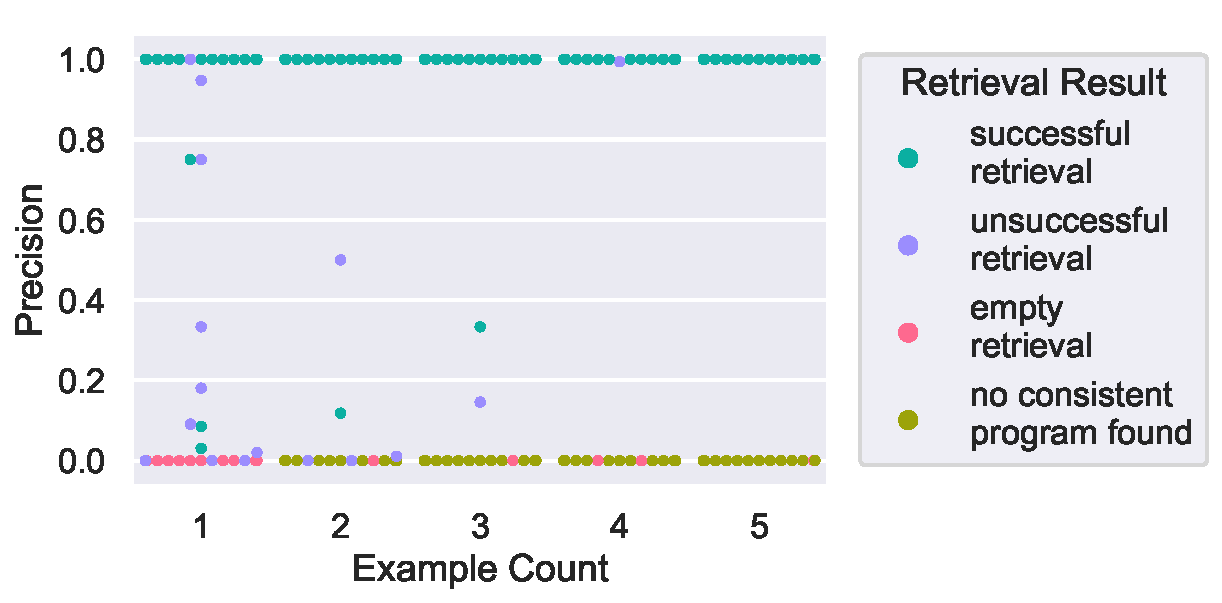
\includegraphics[width=\textwidth, clip]{img/big-study/precision-extraction-result-PBE.pdf}
		\caption{Precision of PBE Chunk Retrieval Results Compared with Example Count}
		\label{fig:precision-extraction-result-PBE}
	\end{minipage}\hfill
	\begin{minipage}{0.45\textwidth}
		\centering
		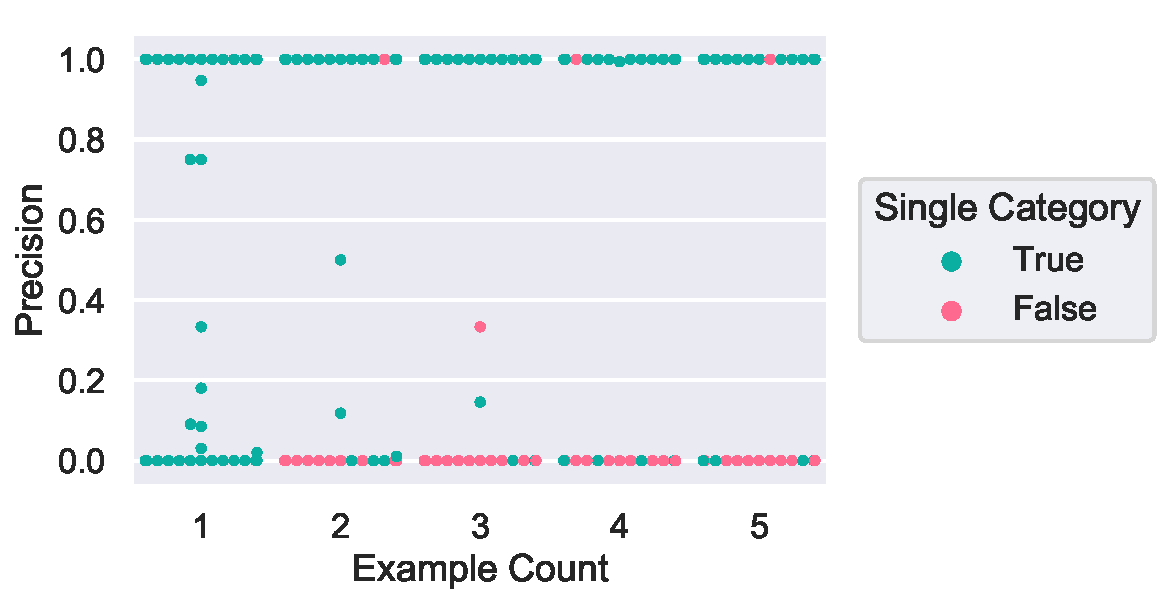
\includegraphics[width=\textwidth, clip]{img/big-study/precision-singlecategory-swarm-PBE.pdf}
		\caption{Precision of PBE Chunk Retrieval Compare with Example Count and Category Singularity}
		\label{fig:precision-singlecategory-swarm-PBE}
	\end{minipage}
\end{figure}
\subsection{Regular Expression Program Synthesis by Example (PBE)}
Out of the 400 runs in our evaluation, 5 runs per each of the 80 example sets, PBE extracted all the desired lines in 138 cases.
Figure \ref{fig:failure-reason-PBE} shows that in 89 cases a program was successfully synthesized, though in 59 cases the synthesized program yielded no output at all.
In 30 cases the synthesized program did not extract all of the desired lines, though still had an average recall of 28\%.
In 173 cases the PROSE program synthesis could not synthesize a singular regular expression program that satisfies all of the configuring examples.

Figure \ref{fig:failure-reason-categorycount-PBE} shows that the success of the program syntesis algorithm highly depends on the structural categories present in the configuring examples.
Programs could only be synthesized if at maximum two categories were present.

More than three examples yield no improvement in the precision of PBE chunk retrieval, as you can see in Figures \ref{fig:precision-extraction-result-PBE} and \ref{fig:precision-singlecategory-swarm-PBE}.

% \begin{figure}[htbp]
% 	\centering
% 	\begin{minipage}{0.45\textwidth}
% 		\centering
% 		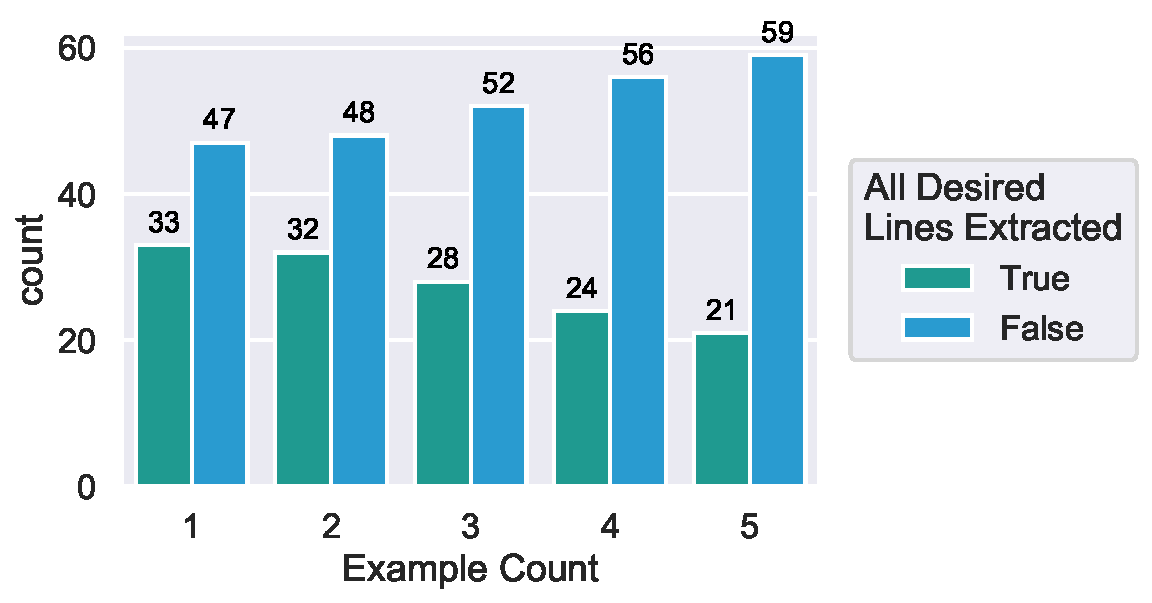
\includegraphics[width=\textwidth, clip]{img/big-study/success-examples-PBE.pdf}
% 		\caption{Successful Extractions per Number of Examples for PBE}
% 		\label{fig:success-examples-pbe}
% 	\end{minipage}\hfill
% 	\begin{minipage}{0.45\textwidth}
% 		\centering
% 		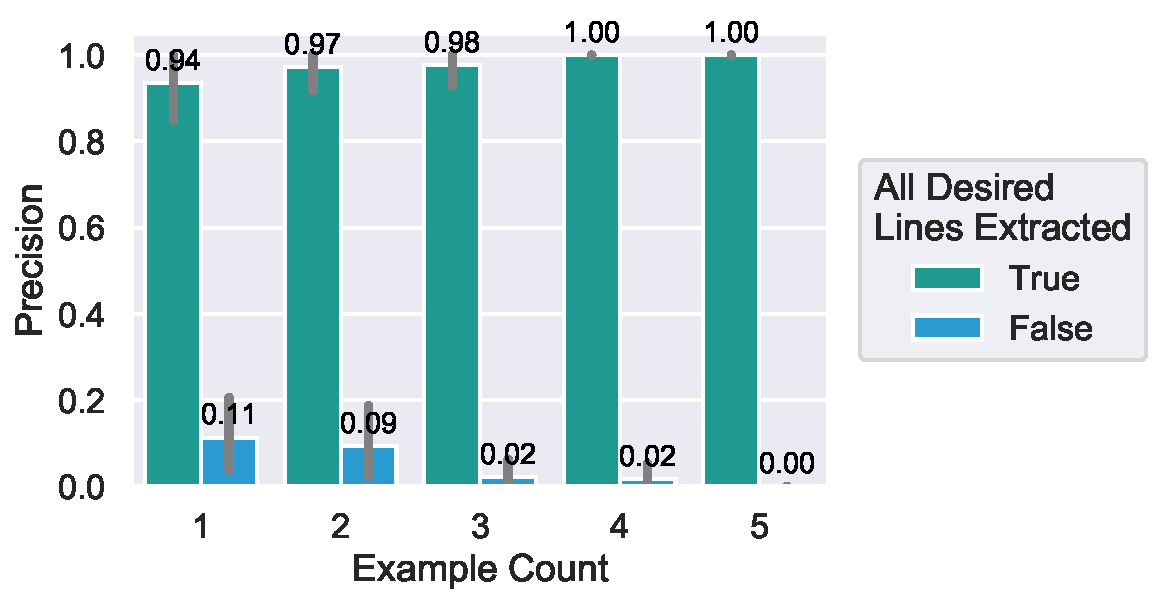
\includegraphics[width=\textwidth, clip]{img/big-study/precision-PBE.pdf}
% 		\caption{Precision of Extractions per Number of Examples for PBE}
% 		\label{fig:precision-pbe}
% 	\end{minipage}
% \end{figure}
% \begin{figure}[htbp]
% 	\centering
% 	\begin{minipage}{0.45\textwidth}
% 		\centering
% 		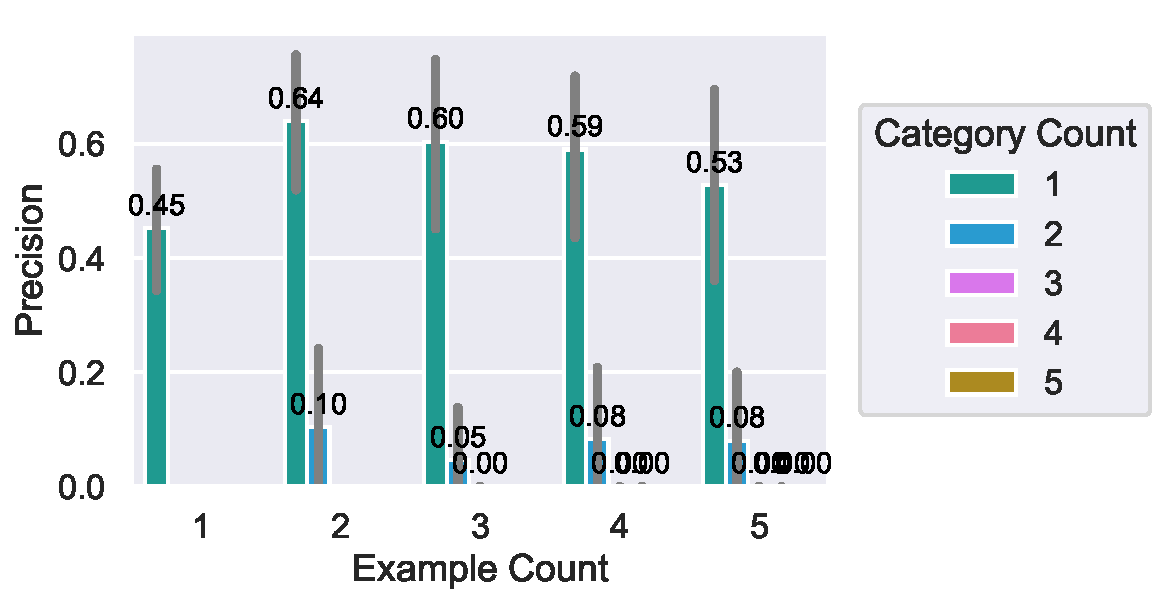
\includegraphics[width=\textwidth, clip]{img/big-study/precision-categorycount-examplecount-PBE.pdf}
% 		\caption{Precision of PBE Extractions by CategoryCount}
% 		\label{fig:precision-categorycount-examplecount-pbe}
% 	\end{minipage}\hfill
% 	\begin{minipage}{0.45\textwidth}
% 		\centering
% 		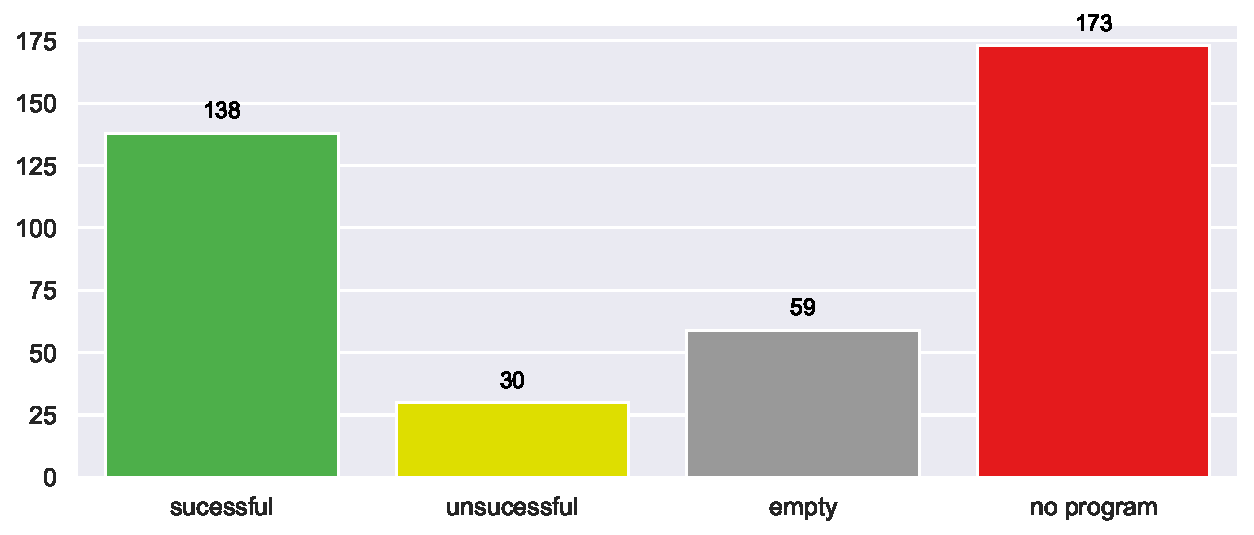
\includegraphics[width=\textwidth, clip]{img/big-study/failure-reason-PBE.pdf}
% 		\caption{Reasons for PBE Runs to Fail}
% 		\label{fig:failure-reason-pbe}
% 	\end{minipage}
% \end{figure}

% This section addresses the results produced by the PBE technique in our study.
% We start by comparing success rate and precision for different example counts and showing the influence of example categories.
% Next we go into detail in which cases pbe fails
% \subsubsection{Success-Rate}
% \subsubsection{Precision}
% \subsubsection{Example Categories}
% \subsubsection{Specific Failure Reasons}
% \todo{FAILURE REASON AGAINST EXAMPLE CATEGORIES}
% \subsection{Successful Extractions}
% successful is interpreted by us as: all lines that were desired (within our oracle) were also extracted during the test

% Figure \ref{fig:success-all} shows how successful the four different tecnhiques were in our study.
% Figure \ref{fig:success-examples-pbe} shows that the success rate for PBE decreases with increasing example count for pbe. Section \ref{TODO ref to pbe section} explains in more detail whi this fails
% Figure \ref{fig:success-examples-ts} shows that the success rate for TS varies but stays roughly the same for different example counts
% Figure \ref{fig:success-examples-skws} shows that the success rate for KWS varies but stays roughly the same for different example counts
% Figure \ref{fig:success-examples-pbe} shows that 

\subsection{Common Text Similarity (CTS)}

% \begin{figure}[htbp]
% 	\centering
% 	\begin{minipage}{0.45\textwidth}
% 		\centering
% 		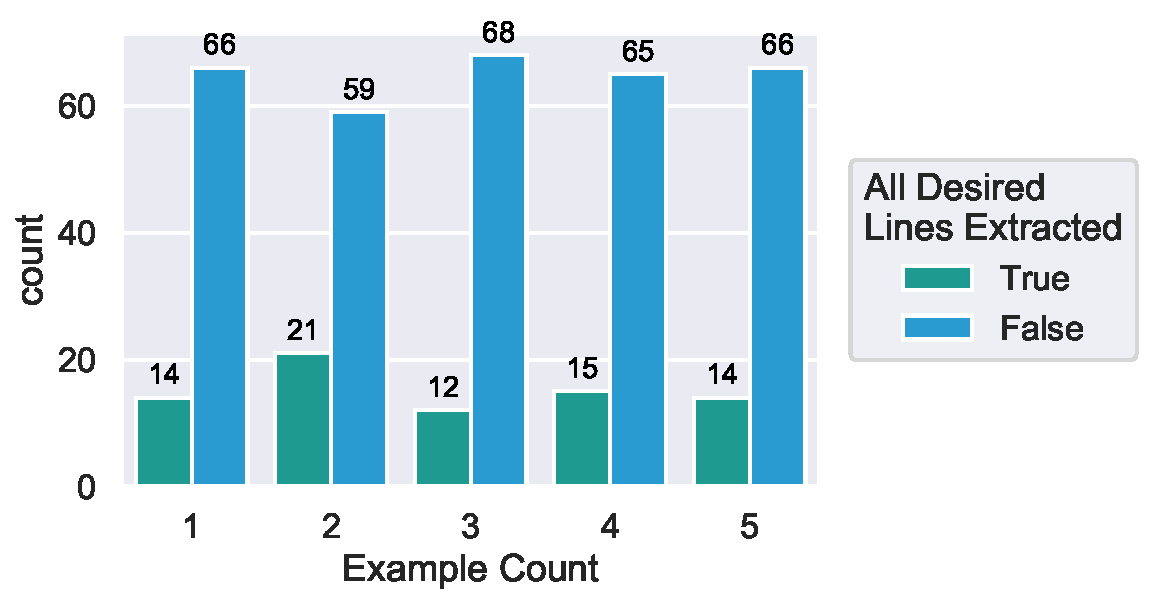
\includegraphics[width=\textwidth, clip]{img/big-study/success-examples-TS.pdf}
% 		\caption{Successful Extractions per Number of Examples for TS}
% 		\label{fig:success-examples-ts}
% 	\end{minipage}\hfill
% 	\begin{minipage}{0.45\textwidth}
% 		\centering
% 		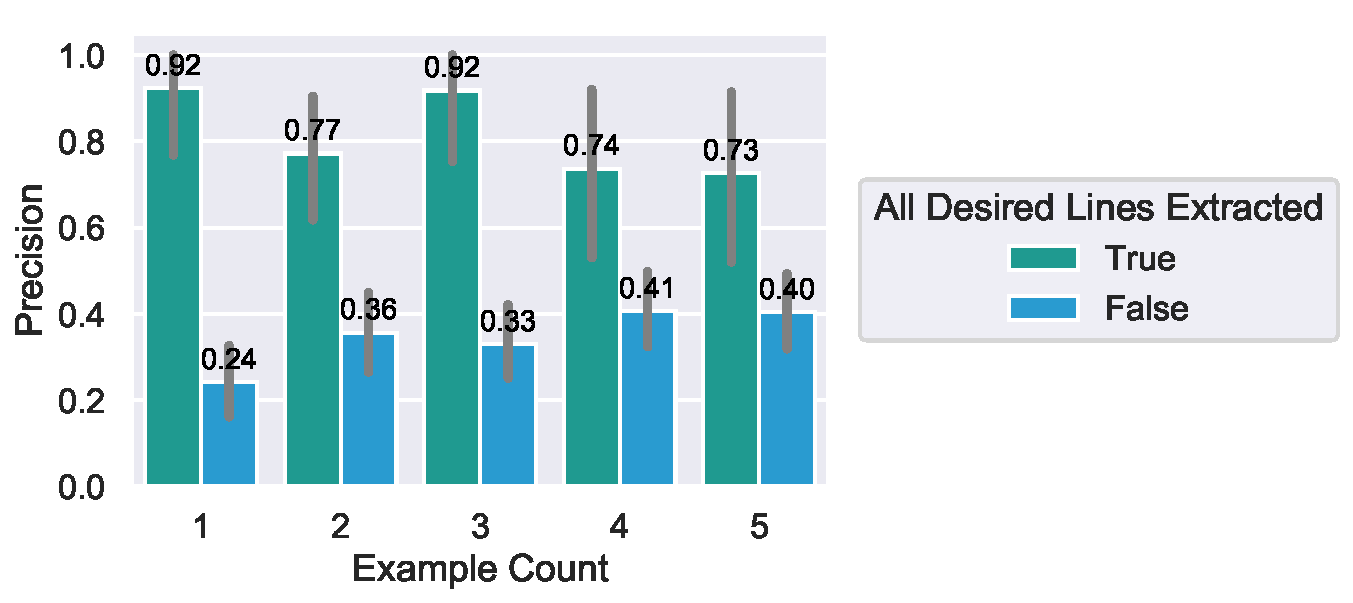
\includegraphics[width=\textwidth, clip]{img/big-study/precision-TS.pdf}
% 		\caption{Precision of Extractions per Number of Examples for TS}
% 		\label{fig:precision-ts}
% 	\end{minipage}
% \end{figure}
% \begin{figure}[htbp]
% 	\centering
% 	\begin{minipage}{0.45\textwidth}
% 		\centering
% 		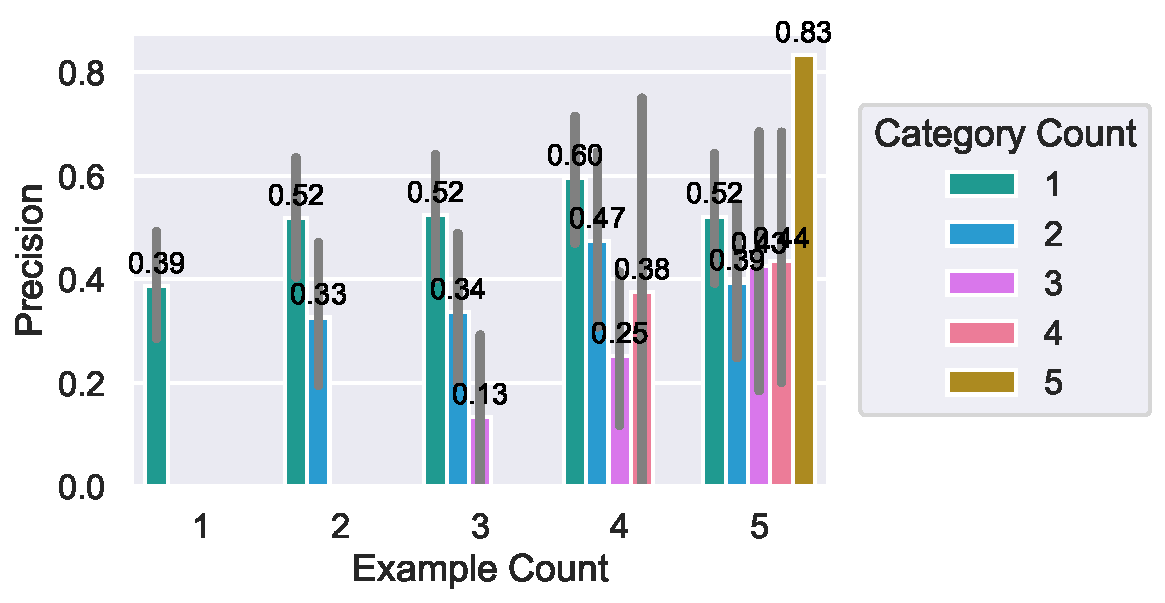
\includegraphics[width=\textwidth, clip]{img/big-study/precision-categorycount-examplecount-TS.pdf}
% 		\caption{Precision of TS Extractions by CategoryCount}
% 		\label{fig:precision-categorycount-examplecount-ts}
% 	\end{minipage}\hfill
% 	\begin{minipage}{0.45\textwidth}
% 		\centering
% 		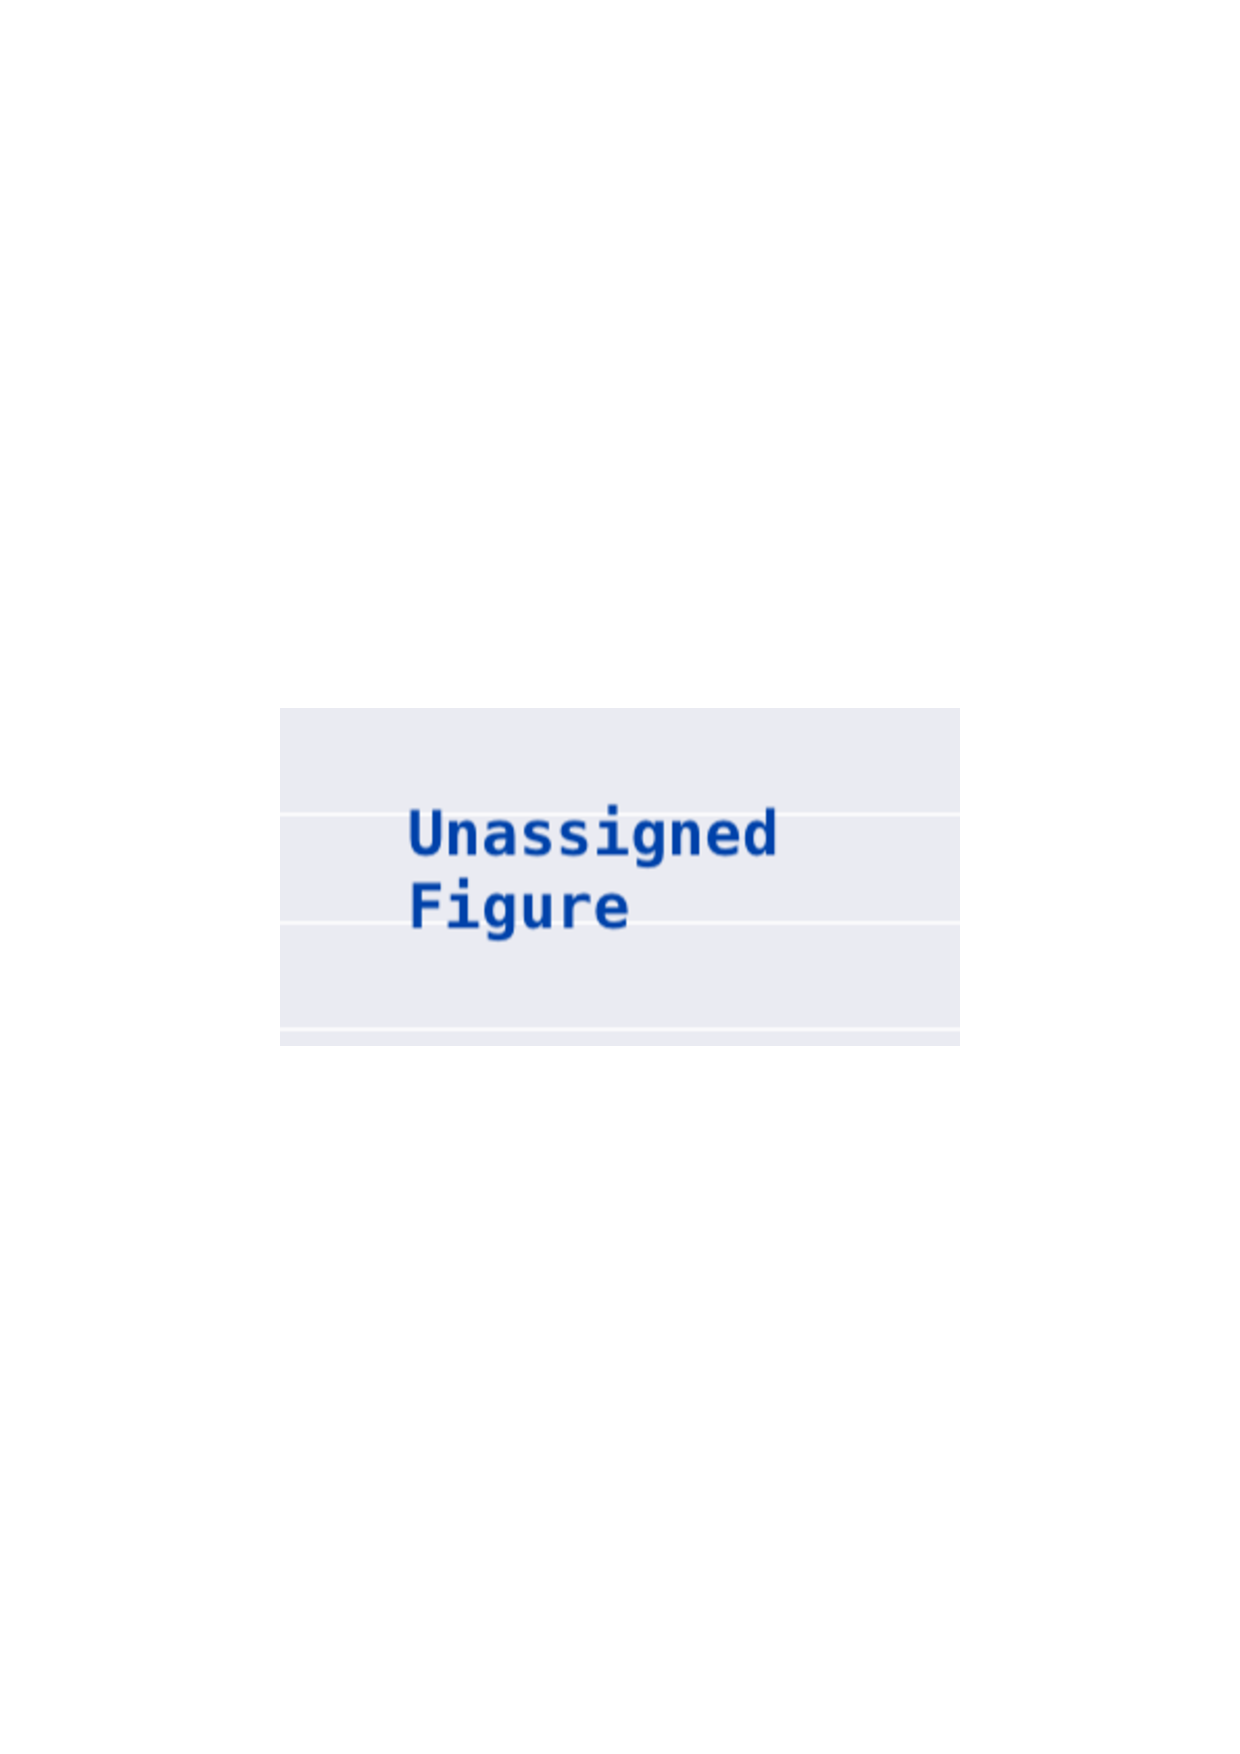
\includegraphics[width=\textwidth, clip]{img/big-study/xxx.pdf}
% 		\caption{xxx}
% 		\label{fig:xxx}
% 	\end{minipage}
% \end{figure}

% \subsubsection{Success-Rate}
% \subsubsection{Precision}
% \subsubsection{Example Categories}


\subsection{Keyword Search (KWS)}

% \begin{figure}[htbp]
% 	\centering
% 	\begin{minipage}{0.45\textwidth}
% 		\centering
% 		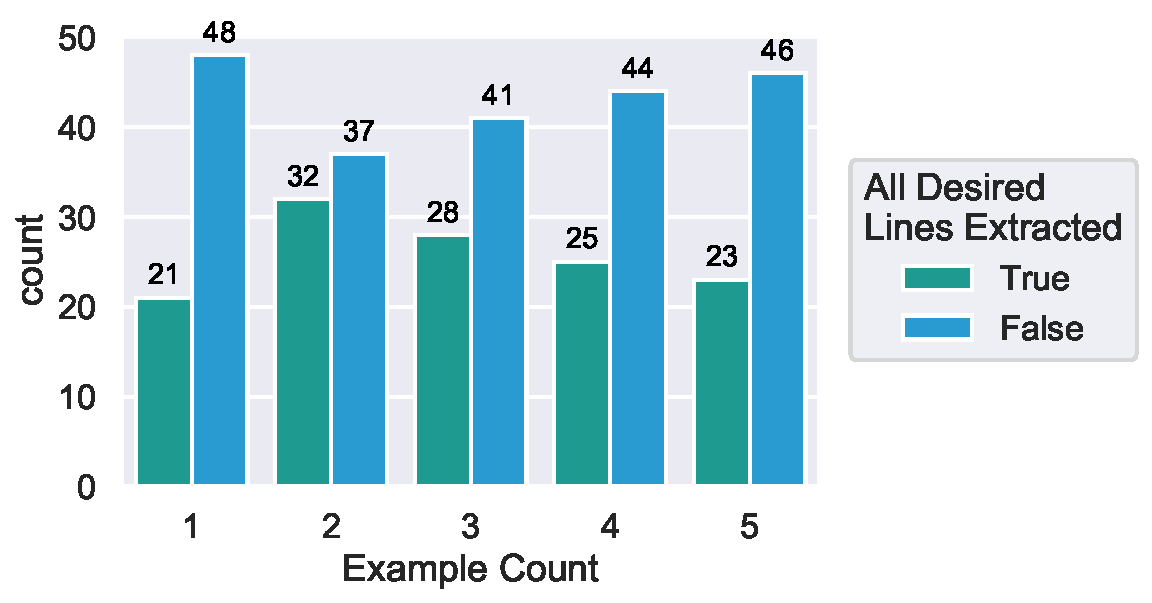
\includegraphics[width=\textwidth, clip]{img/big-study/success-examples-SKWS.pdf}
% 		\caption{Successful Extractions per Number of Examples for SKWS}
% 		\label{fig:success-examples-skws}
% 	\end{minipage}\hfill
% 	\begin{minipage}{0.45\textwidth}
% 		\centering
% 		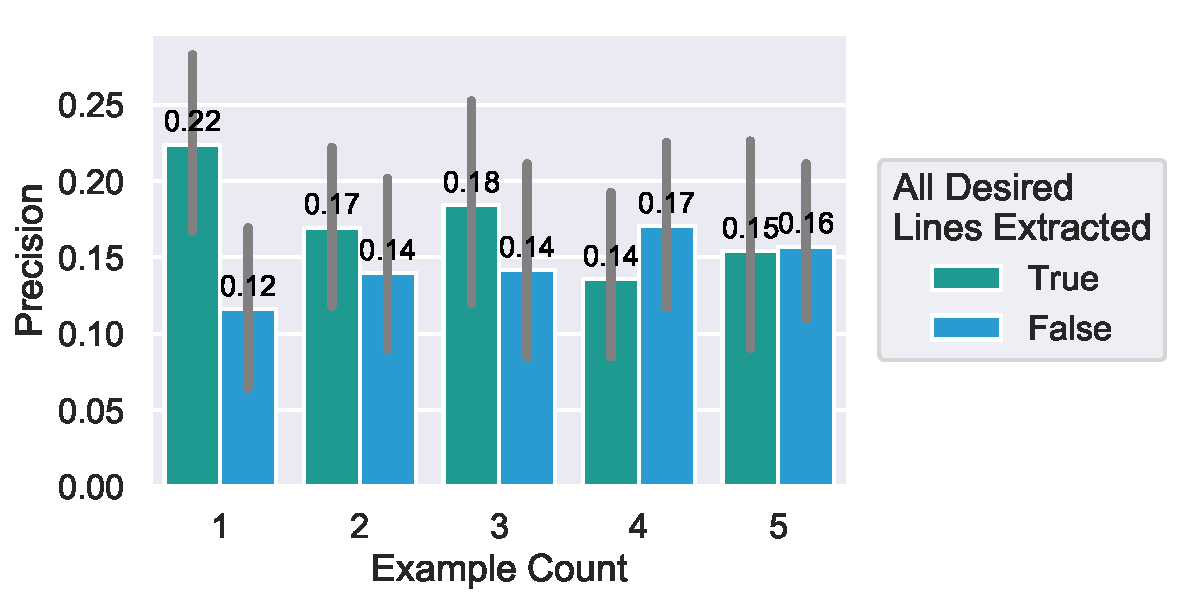
\includegraphics[width=\textwidth, clip]{img/big-study/precision-SKWS.pdf}
% 		\caption{Precision of Extractions per Number of Examples for SKWS}
% 		\label{fig:precision-skws}
% 	\end{minipage}
% \end{figure}
% \begin{figure}[htbp]
% 	\centering
% 	\begin{minipage}{0.45\textwidth}
% 		\centering
% 		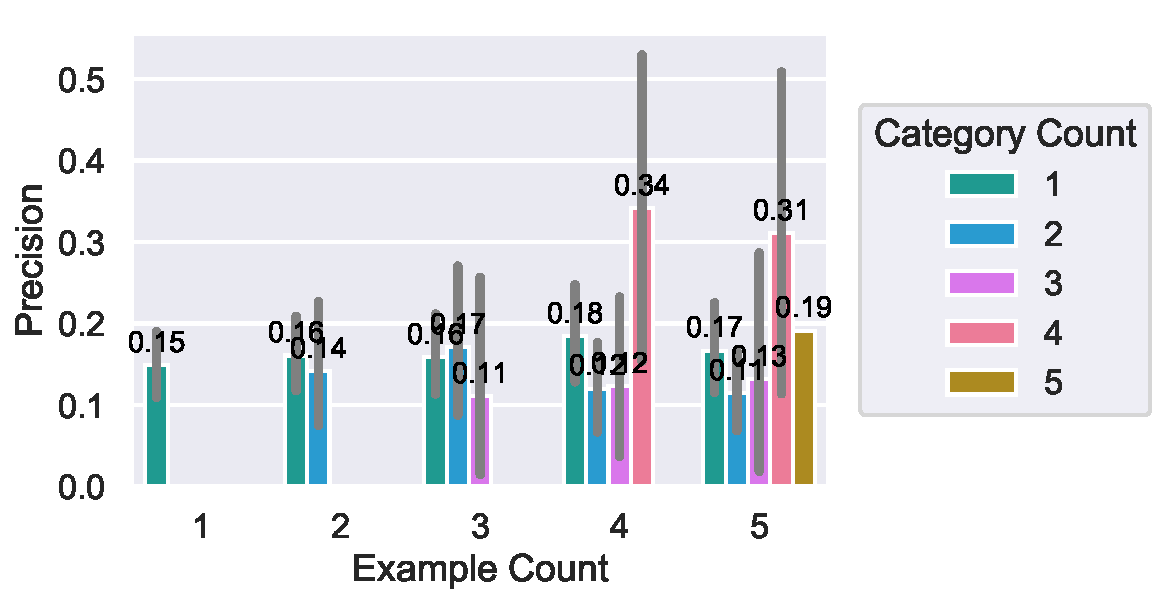
\includegraphics[width=\textwidth, clip]{img/big-study/precision-categorycount-examplecount-SKWS.pdf}
% 		\caption{Precision of SKWS Extractions by CategoryCount}
% 		\label{fig:precision-categorycount-examplecount-skws}
% 	\end{minipage}\hfill
% 	\begin{minipage}{0.45\textwidth}
% 		\centering
% 		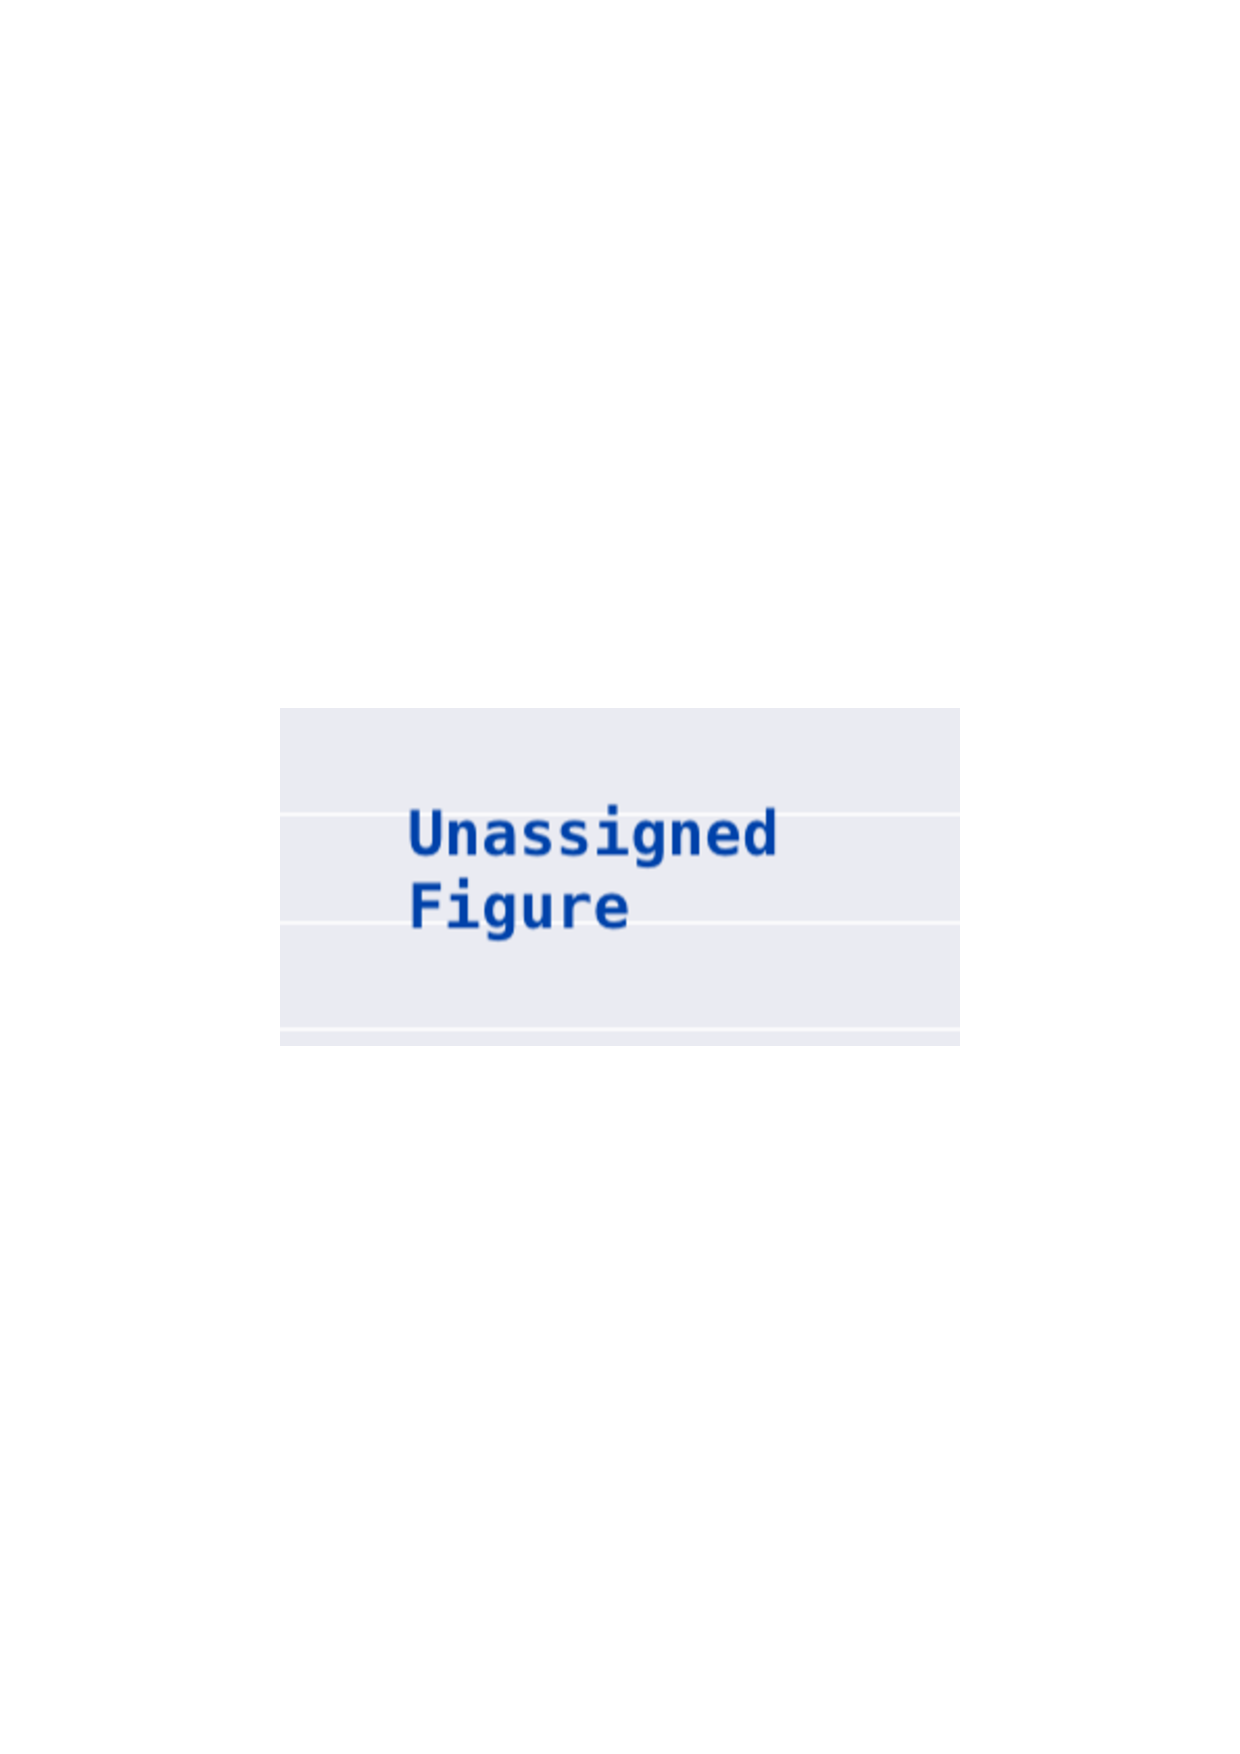
\includegraphics[width=\textwidth, clip]{img/big-study/xxx.pdf}
% 		\caption{xxx}
% 		\label{fig:xxx}
% 	\end{minipage}
% \end{figure}

% \subsubsection{Success-Rate}
% \subsubsection{Precision}
% \subsubsection{Example Categories}


% \subsection{Random Line Retrieval (RLR)}

% \begin{figure}[htbp]
% 	\centering
% 	\begin{minipage}{0.45\textwidth}
% 		\centering
% 		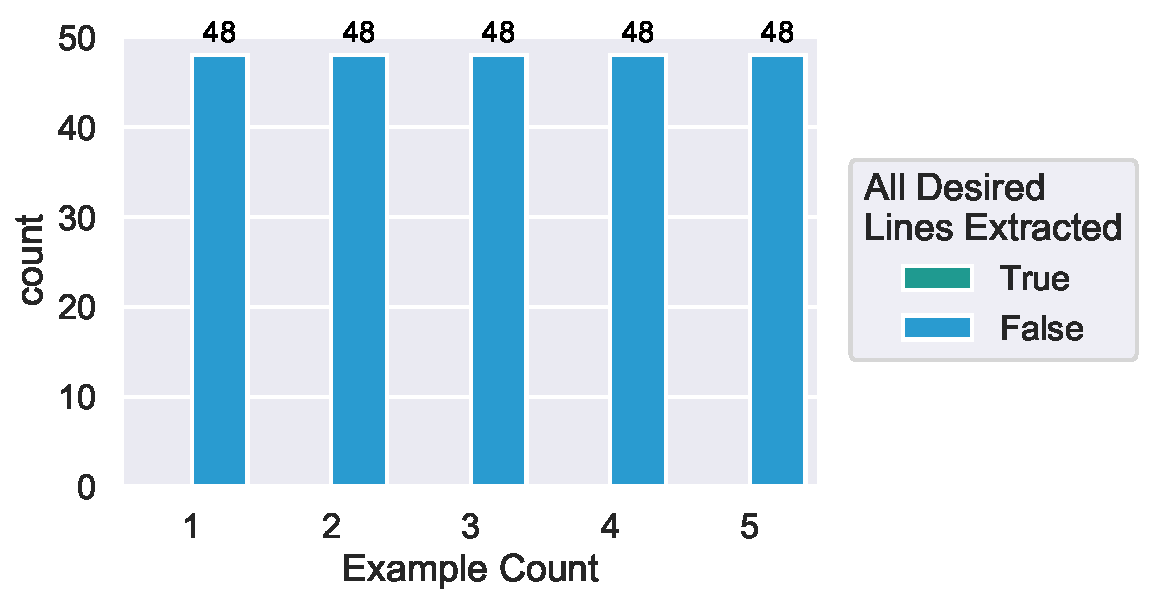
\includegraphics[width=\textwidth, clip]{img/big-study/success-examples-RLR.pdf}
% 		\caption{Successful Extractions per Number of Examples for RLR}
% 		\label{fig:success-examples-rlr}
% 	\end{minipage}\hfill
% 	\begin{minipage}{0.45\textwidth}
% 		\centering
% 		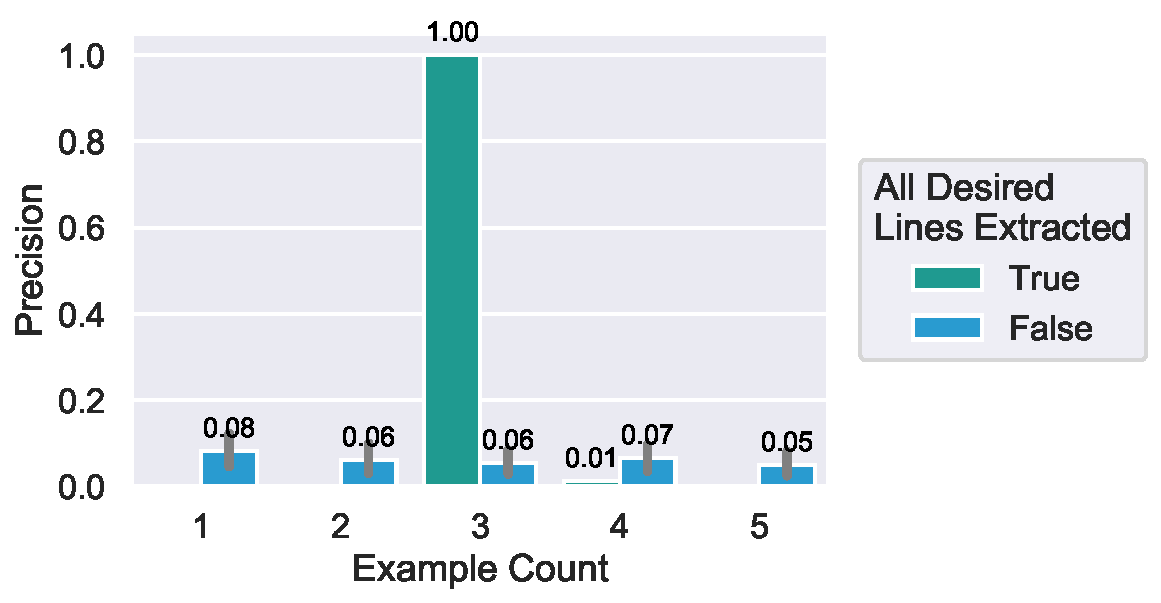
\includegraphics[width=\textwidth, clip]{img/big-study/precision-RLR.pdf}
% 		\caption{Precision of Extractions per Number of Examples for RLR}
% 		\label{fig:precision-rlr}
% 	\end{minipage}
% \end{figure}
% \begin{figure}[htbp]
% 	\centering
% 	\begin{minipage}{0.45\textwidth}
% 		\centering
% 		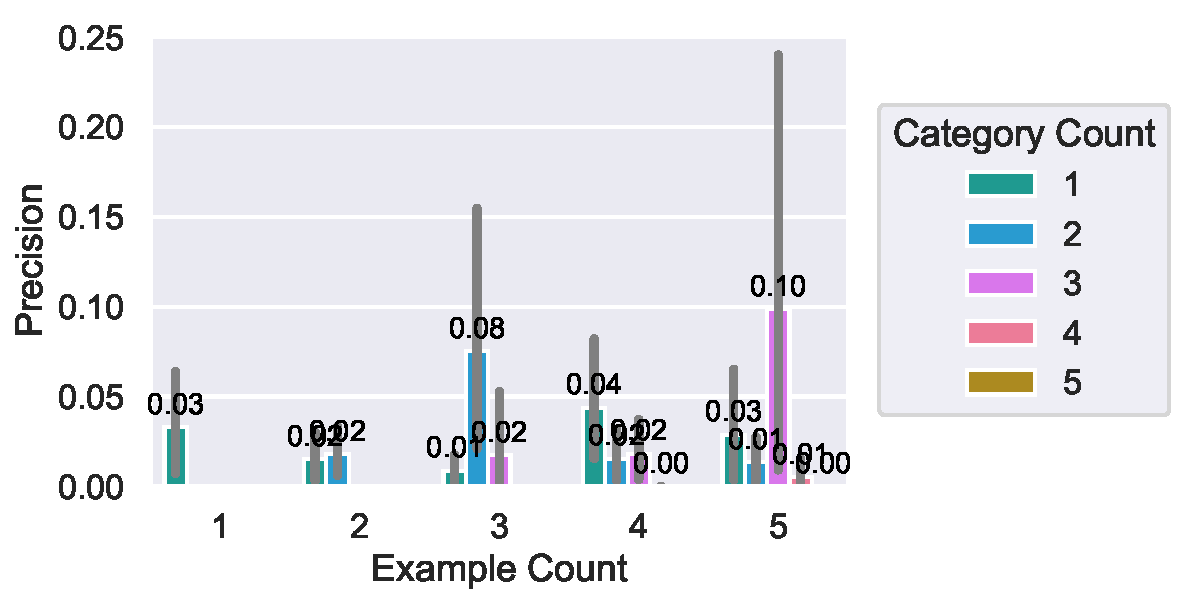
\includegraphics[width=\textwidth, clip]{img/big-study/precision-categorycount-examplecount-RLR.pdf}
% 		\caption{Precision of RLR Extractions by CategoryCount}
% 		\label{fig:precision-categorycount-examplecount-rlr}
% 	\end{minipage}\hfill
% 	\begin{minipage}{0.45\textwidth}
% 		\centering
% 		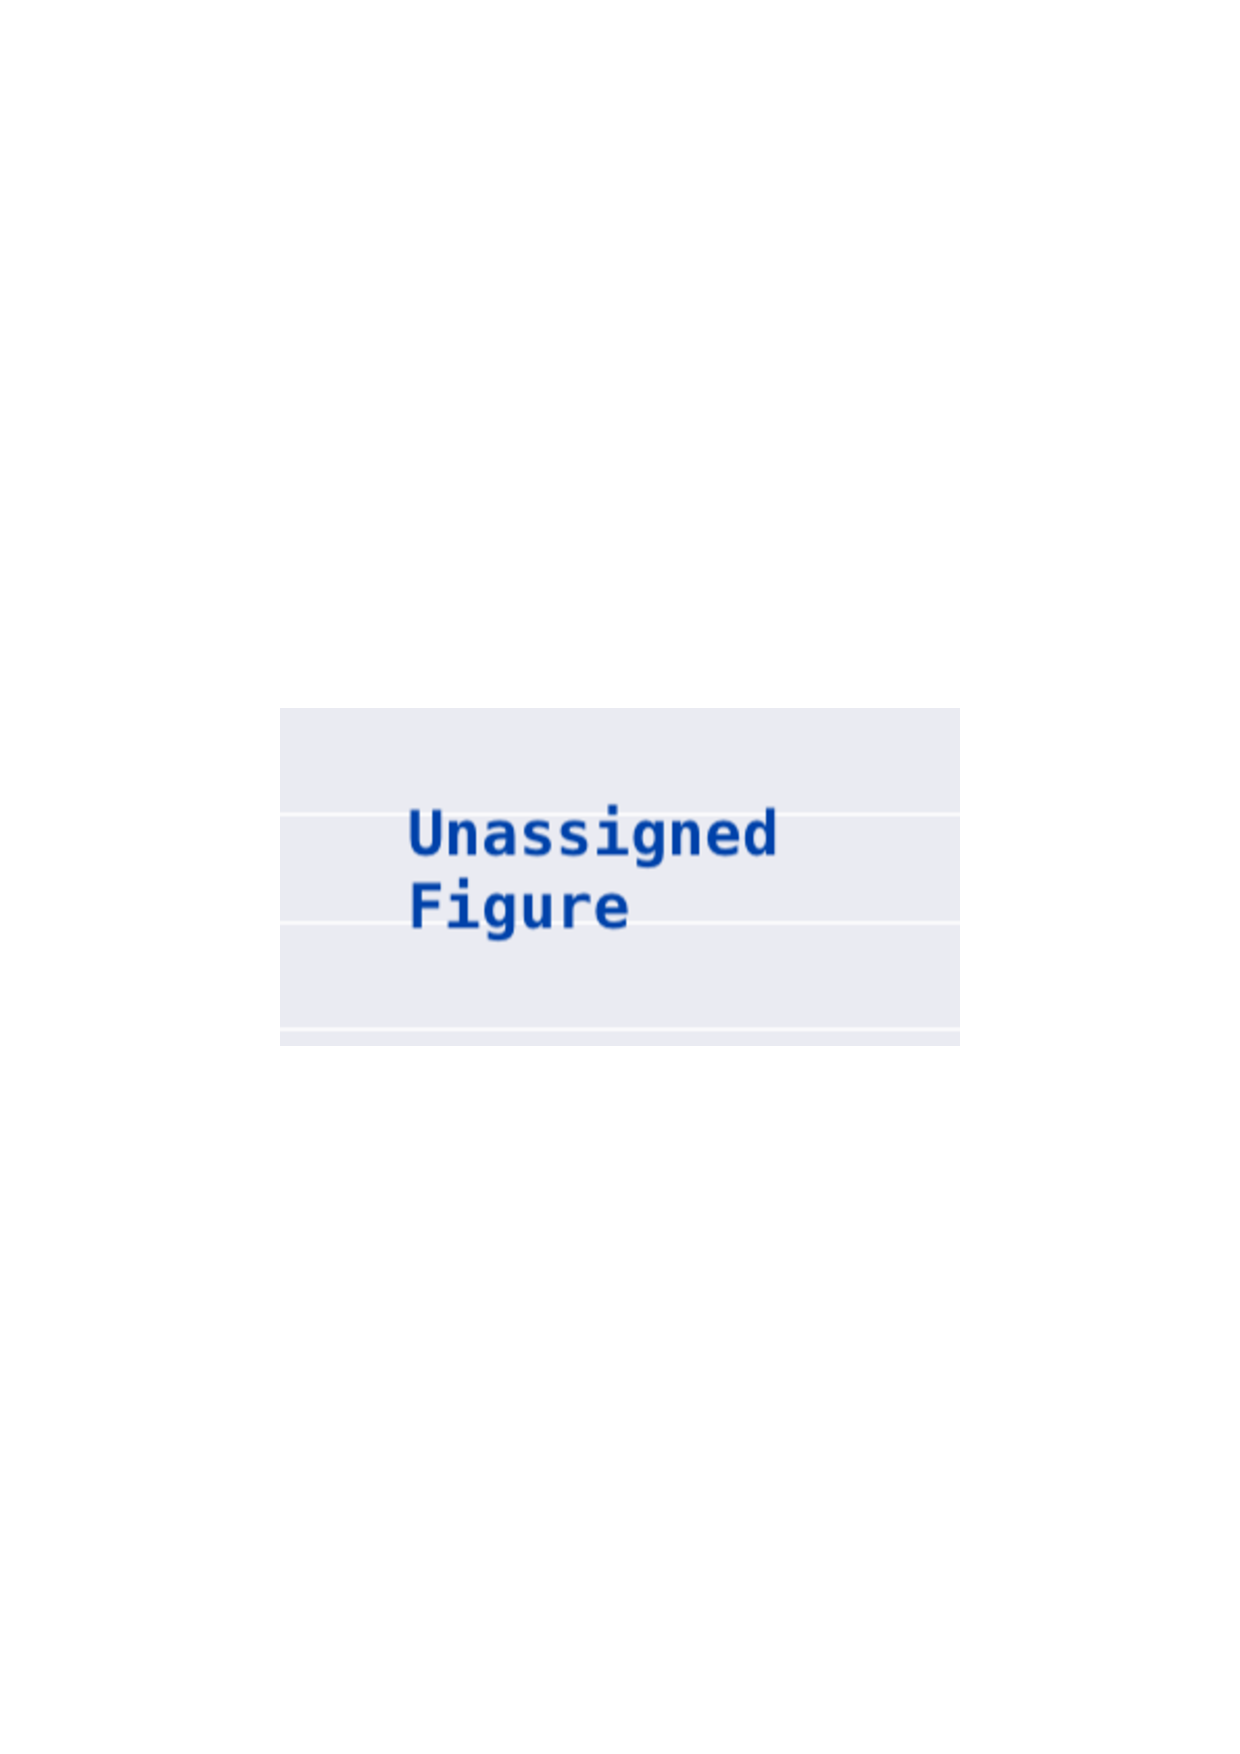
\includegraphics[width=\textwidth, clip]{img/big-study/xxx.pdf}
% 		\caption{xxx}
% 		\label{fig:xxx}
% 	\end{minipage}
% \end{figure}

% For completion this section reports the results for the random line retrieval technique, explained in detail in Section \ref{sec:}

% \subsubsection{Success-Rate}
% \subsubsection{Precision}
% \subsubsection{Example Categories}

\subsection{Comparing All Techniques}
% \begin{figure}[htbp]
% 	\centering
% 	\begin{minipage}{0.45\textwidth}
% 		\centering
% 		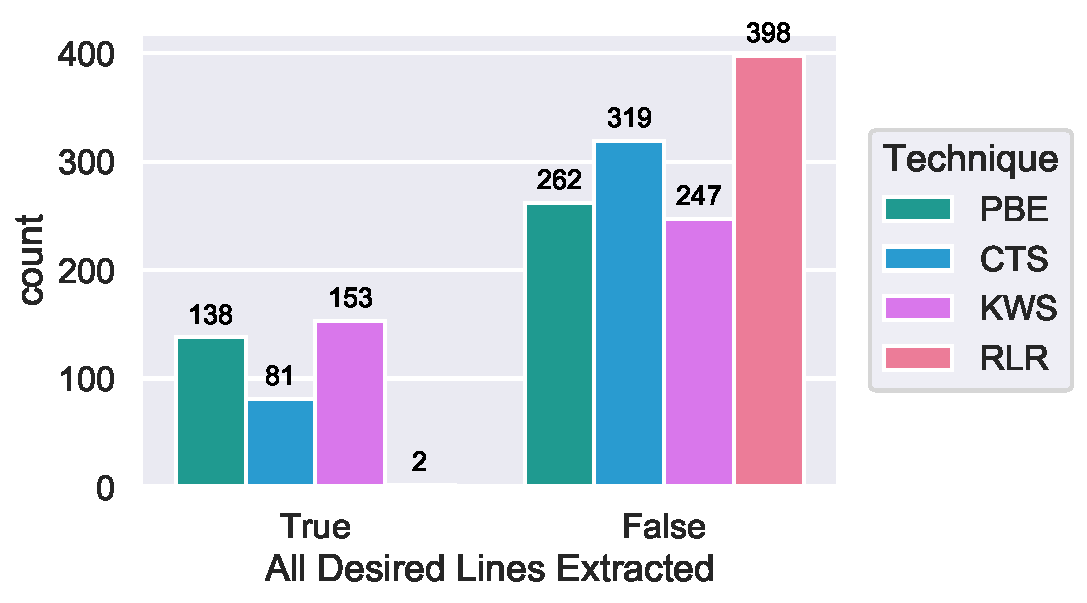
\includegraphics[width=\textwidth, clip]{img/big-study/success-all.pdf}
% 		\caption{Successful Extractions for all Techniques Compared}
% 		\label{fig:success-all}
% 	\end{minipage}\hfill
% 	\begin{minipage}{0.45\textwidth}
% 		\centering
% 		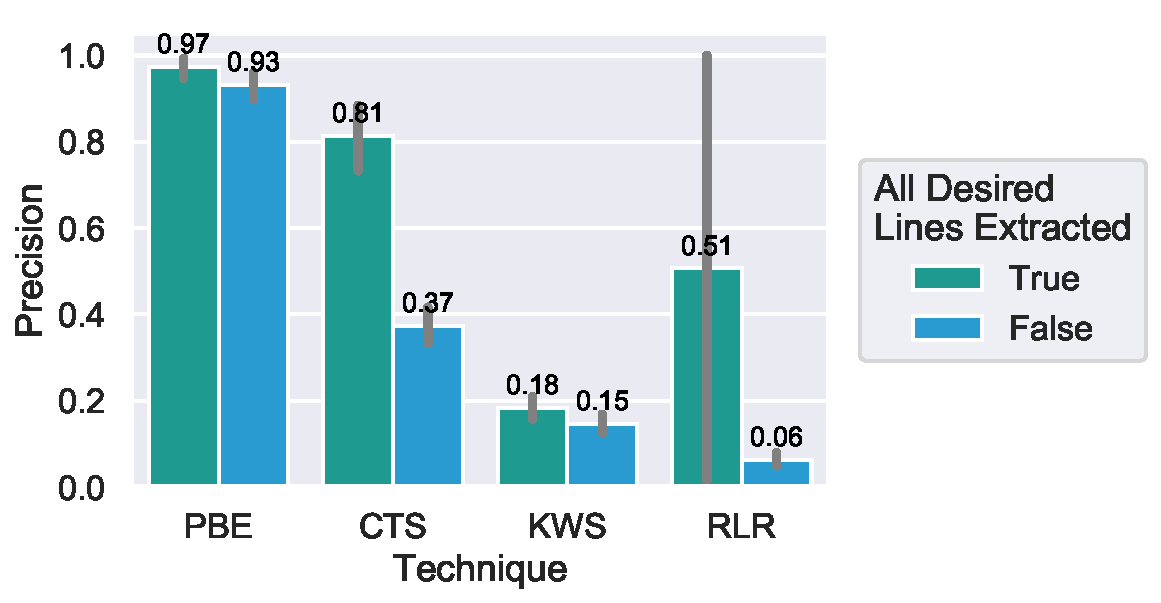
\includegraphics[width=\textwidth, clip]{img/big-study/precision-all.pdf}
% 		\caption{Precision of Extractions for all Techniques Compared}
% 		\label{fig:precision-all}
% 	\end{minipage}
% \end{figure}

% \begin{figure}[htbp]
% 	\centering
% 	\begin{minipage}{0.45\textwidth}
% 		\centering
% 		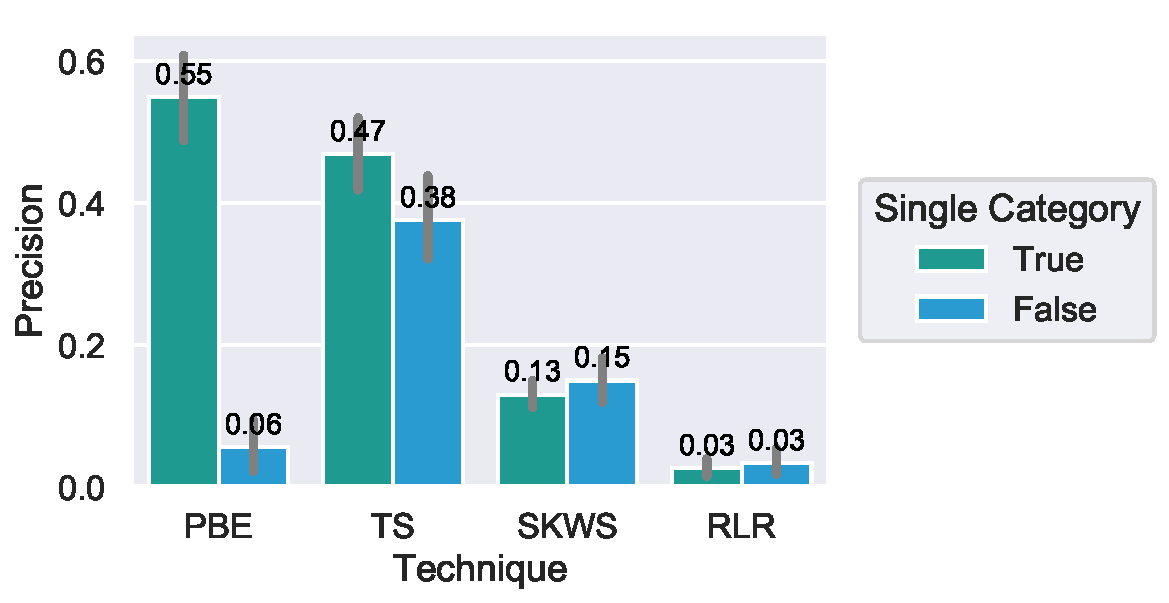
\includegraphics[width=\textwidth, clip]{img/big-study/precision-category-singularity-all.pdf}
% 		\caption{\todo{todo}}
% 		\label{fig:precision-category-singularity-all}
% 	\end{minipage}\hfill
% 	\begin{minipage}{0.45\textwidth}
% 		\centering
% 		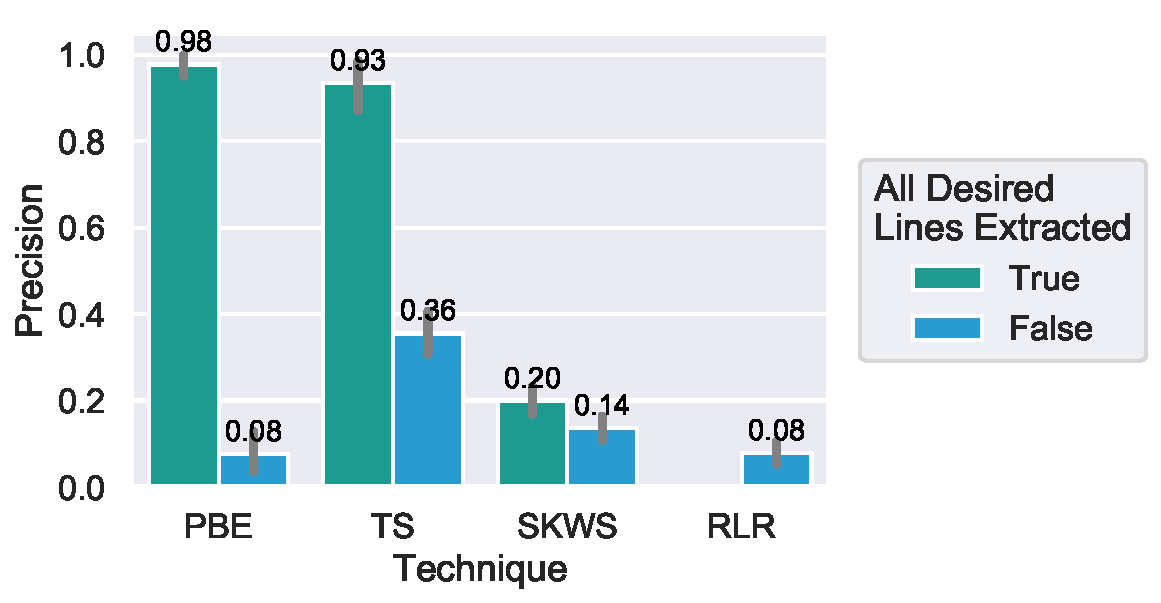
\includegraphics[width=\textwidth, clip]{img/big-study/single-cateogry-precision-all.pdf}
% 		\caption{\todo{todo}}
% 		\label{fig:single-cateogry-precision-all}
% 	\end{minipage}
% \end{figure}

% \begin{figure}[htbp]
% 	\centering
% 	\begin{minipage}{0.45\textwidth}
% 		\centering
% 		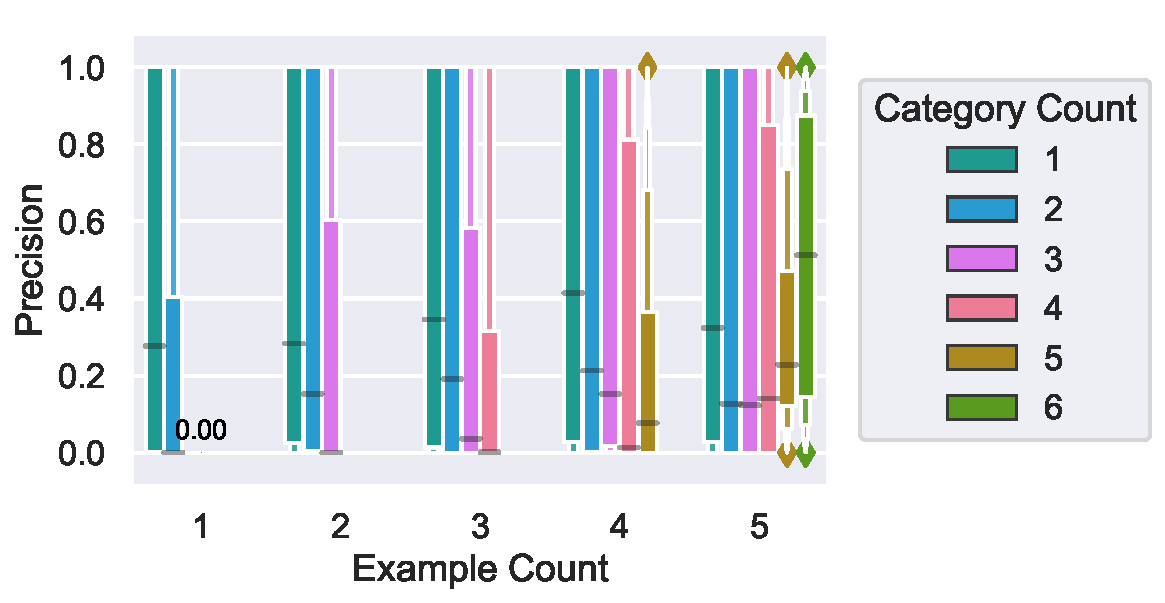
\includegraphics[width=\textwidth, clip]{img/big-study/precision-categorycount-examplecount-all.pdf}
% 		\caption{\todo{todo}}
% 		\label{fig:precision-categorycount-examplecount-all}
% 	\end{minipage}\hfill
% 	\begin{minipage}{0.45\textwidth}
% 		\centering
% 		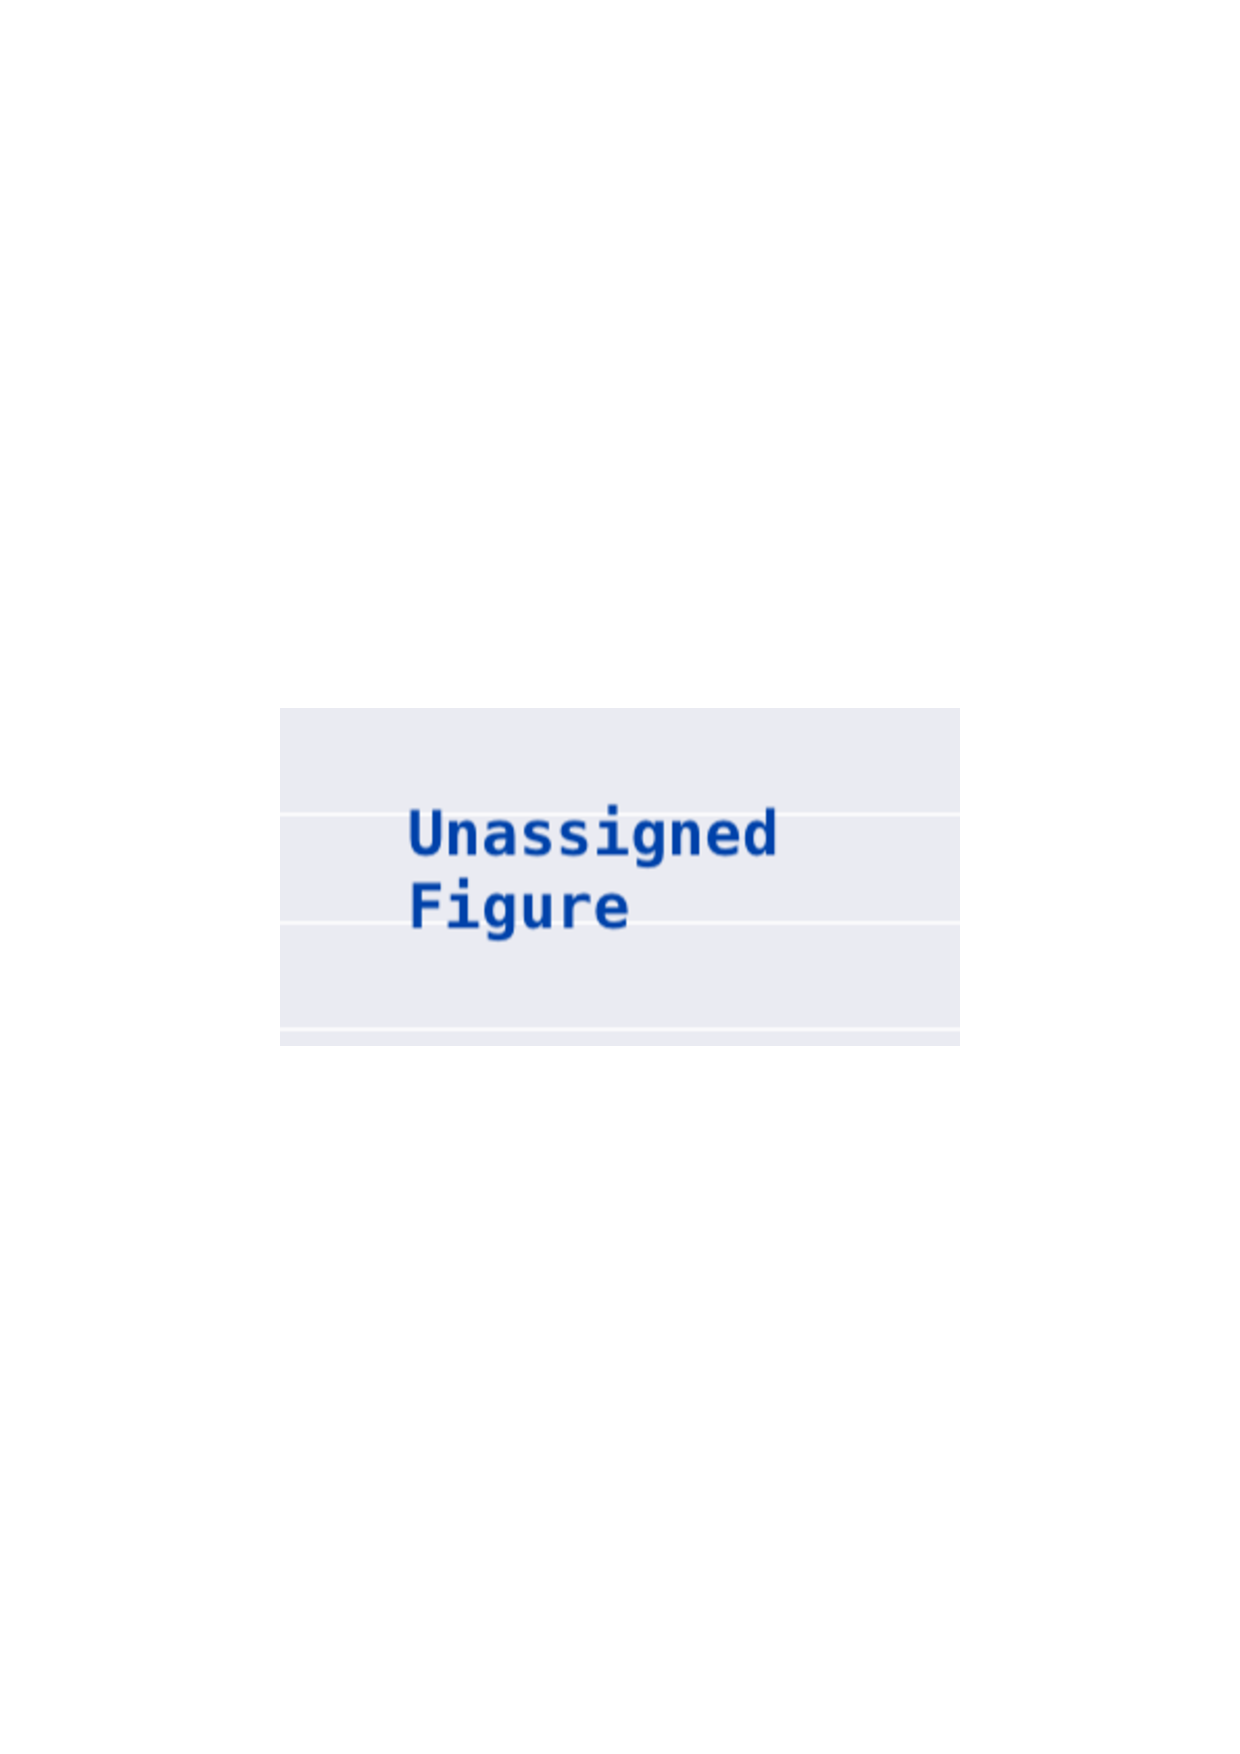
\includegraphics[width=\textwidth, clip]{img/big-study/xxx.pdf}
% 		\caption{\todo{todo}}
% 		\label{fig:xxx}
% 	\end{minipage}
% \end{figure}

% \subsubsection{Success-Rate}
% \subsubsection{Precision}
% \subsubsection{Example Categories}

% \section{Discussion}
% \todo{draw decision tree}

% interpret results - when should PROSE be used? - when should text similarity be used? - when should keyword search be used? - answer RQ about PROSE \& other techniques
\section{Threats to Validity}
%chronologically selected examples -> very specific view



\end{document}
